
\PassOptionsToPackage{unicode}{hyperref}
\PassOptionsToPackage{naturalnames}{hyperref}

\documentclass[tg]{mdtufsm}
\usepackage[brazilian]{babel}

\usepackage[T1]{fontenc}
\usepackage[utf8]{inputenc}

\usepackage{fix-cm}
\usepackage{times}
\usepackage{graphicx}
\usepackage{array}
\usepackage{listings}
\usepackage{tabularx}
\usepackage{hhline}
\usepackage{amsmath,latexsym,amssymb}
\usepackage{siunitx}
\usepackage{pdfpages}
\usepackage[inner=30mm,outer=20mm,top=30mm,bottom=20mm]{geometry}
\usepackage{subcaption}

\lstdefinelanguage{Java}{
    keywords={public, private, new, true, boolean, false, catch, void, return, null, for, switch, var, if, in, while, else, case, break, class, Funcionalidade, Contexto, Dado, Quando, E, Entao, Cenario, Delineacao, Exemplos},
    keywordstyle=\color[rgb]{0.2,0.4,0.55}\bfseries,
    ndkeywords={export, throw, implements, import, this, @Before, @Test, @After, @Dado, @Quando, @E, @Entao, @Documented, @Retention, @Target, @Teste, @aceitacao, @rejeicao, codigoDis, nomeNovaDisciplina, relevancia, siglaInst, msgErro},
    %ndkeywords={Add, Num},
    ndkeywordstyle=\color[RGB]{218,202,66}\bfseries,
    %identifierstyle=\color{black},
    sensitive=true,
    comment=[l]{//},
    morecomment=[s]{/*}{*/},
    commentstyle=\color{purple}\ttfamily,
    % stringstyle=\color[rgb]{0.0,0.4,0.65}\ttfamily,
    stringstyle=\color[RGB]{34,128,24}\ttfamily,
    %morestring=[b]',
    morestring=[b]"
}

\lstset{
	language=Java,
	basicstyle=\tiny,
	commentstyle=\color[rgb]{0,0.2,0}\normalfont,
	frame=single,
	%texcl=true,
	numbers=left,
	showstringspaces=false,
}

\lstset{
	basicstyle=\scriptsize\ttfamily,
	tabsize=2,
	frame=single,
	breaklines=true,
	breakatwhitespace=true,
	xleftmargin=0cm,
	xrightmargin=0cm,
	literate=
		{á}{{\'a}}1 {é}{{\'e}}1 {í}{{\'i}}1 {ó}{{\'o}}1 {ú}{{\'u}}1
		{Á}{{\'A}}1 {É}{{\'E}}1 {Í}{{\'I}}1 {Ó}{{\'O}}1 {Ú}{{\'U}}1
		{à}{{\`a}}1 {è}{{\`e}}1 {ì}{{\`i}}1 {ò}{{\`o}}1 {ù}{{\`u}}1
		{À}{{\`A}}1 {È}{{\'E}}1 {Ì}{{\`I}}1 {Ò}{{\`O}}1 {Ù}{{\`U}}1
		{ä}{{\"a}}1 {ë}{{\"e}}1 {ï}{{\"i}}1 {ö}{{\"o}}1 {ü}{{\"u}}1
		{Ä}{{\"A}}1 {Ë}{{\"E}}1 {Ï}{{\"I}}1 {Ö}{{\"O}}1 {Ü}{{\"U}}1
		{â}{{\^a}}1 {ê}{{\^e}}1 {î}{{\^i}}1 {ô}{{\^o}}1 {û}{{\^u}}1
		{Â}{{\^A}}1 {Ê}{{\^E}}1 {Î}{{\^I}}1 {Ô}{{\^O}}1 {Û}{{\^U}}1
		{ã}{{\~a}}1 {Ã}{{\~A}}1 {õ}{{\~o}}1 {Õ}{{\~O}}1
		{ç}{{\c c}}1 {Ç}{{\c C}}1,
	texcl=true,
	%numbers=left,
	showstringspaces=false,
	commentstyle=\normalfont
}

\captionsetup{compatibility=false}
\geometry{a4paper}
\usepackage[hidelinks,
            bookmarksopen=true,linktoc=none,colorlinks=true,
            linkcolor=black,citecolor=black,filecolor=magenta,urlcolor=blue,
            pdftitle={Automação de Interfaces Gráficas para Modelos de Simulação de Culturas Agrícolas com Base em Linguagem de Programação Visual},
            pdfauthor={Romulo Pulcinelli Benedetti},
            pdfsubject={Trabalho de Graduação},
            pdfkeywords={Automação de Software, Linguagens de Programação Visual, Modelos de Simulação de Culturas Agrícolas, Automação de Interfaces Gráficas, Blockly}
           ]{hyperref}

\def\Cpp{{C\nolinebreak[4]\raisebox{.20ex}{\small\bf++}}}
\newcommand{\todo}[1]{}
\graphicspath{{./images/}}
%%=============================================================================
%% Trampa para corrigir o bug do hyperref que redefine o caption das figuras e das
%% tabelas, não colocando o nome ``Figura'' antes do número do mesmo na lista
%%=============================================================================

\makeatletter

\long\def\@caption#1[#2]#3{%
  \expandafter\ifx\csname if@capstart\expandafter\endcsname
                  \csname iftrue\endcsname
    \global\let\@currentHref\hc@currentHref
  \else
    \hyper@makecurrent{\@captype}%
  \fi
  \@ifundefined{NR@gettitle}{%
    \def\@currentlabelname{#2}%
  }{%
    \NR@gettitle{#2}%
  }%
  \par\addcontentsline{\csname ext@#1\endcsname}{#1}{%
    \protect\numberline{\csname fnum@#1\endcsname ~-- }{\ignorespaces #2}%
  }%
  \begingroup
    \@parboxrestore
    \if@minipage
      \@setminipage
    \fi
    \normalsize
    \expandafter\ifx\csname if@capstart\expandafter\endcsname
                    \csname iftrue\endcsname
      \global\@capstartfalse
      \@makecaption{\csname fnum@#1\endcsname}{\ignorespaces#3}%
    \else
      \@makecaption{\csname fnum@#1\endcsname}{%
        \ignorespaces
        \ifHy@nesting
          \expandafter\hyper@@anchor\expandafter{\@currentHref}{#3}%
        \else
          \Hy@raisedlink{%
            \expandafter\hyper@@anchor\expandafter{%
              \@currentHref
            }{\relax}%
          }%
          #3%
        \fi
      }%
    \fi
    \par
  \endgroup
}

\makeatother

%%% END Article customizations

\title{Automação de Interfaces Gráficas para Modelos de Simulação de Culturas Agrícolas com Base em Linguagem de Programação Visual}
\author{Benedetti}{Romulo Pulcinelli}
\course{Curso de Ciência da Computação}
\altcourse{Curso de Ciência da Computação}
\institute{Centro de Tecnologia}
\degree{Bacharel em Ciência da Computação}

\trabalhoNumero{}
\advisor[Profª.]{Drª.}{Charão}{Andrea Schwertner}
\orientadoratrue

\committee[Prof. Dr.]{Streck}{Nereu Augusto}{UFSM}
\committee[Prof. Dr.]{Lima}{João Vicente Ferreira}{UFSM}

\date{06}{Julho}{2016}

\keyword{Automação de Software}
\keyword{Linguagens de Programação Visual}
\keyword{Modelos de Simulação de Culturas Agrícolas}
\keyword{Automação de Interfaces Gráficas}
\keyword{Blockly}

\begin{document}
    \maketitle
    \makeapprove

    \begin{abstract}
        A automação de tarefas é uma forma bastante eficiente pela qual podemos reduzir custos e aumentar a produtividade e qualidade da atividade humana. A computação por si é uma ferramenta para atingir a automação de tarefas, com vários exemplos de softwares focados em automatizar tarefas específicas sob comando do usuário, sendo a automatização destes softwares um campo a parte. Observamos a aproximação destes softwares a abordagens mais naturais ao raciocínio humano, por meio de interfaces gráficas e contextualização dos elementos com base no mundo real, tornando estes softwares menos distantes do paradigma de interação do humano com a realidade. Desta forma este trabalho objetiva abordar a utilização de tecnologias voltadas a programação visual, em especial a biblioteca para criação de linguagens visuais, Blockly, para melhorar a abordagem de automação de tarefas, com foco em softwares gráficos de modelagem matemática agrícola, assim inserindo a atividade de automatizar estes softwares gráficos, dentro do mesmo domínio de abstração que as atividades destes softwares ocorrem.
    \end{abstract}

    \tableofcontents

    \setlength{\baselineskip}{1.5\baselineskip}

    \chapter{Introdução}

    	No desenvolvimento de software, áreas de conhecimento como engenharia de software e qualidade de software investigam processos e normas, com o objetivo de reduzir a quantia de recursos necessários e garantir a qualidade de software produzido. Um dos produtos destas áreas, envolvendo automação, foi o campo de conhecimento de testes de software.

        Sendo que o software pode realizar diversas tarefas, e estas podem assumir diversos estados, qualquer abordagem de teste de software, numa situação ideal deveria avaliar todas estas tarefas e seus estados para fornecer as melhores informações possíveis sobre a qualidade do software, o que facilmente pode se tornar uma tarefa repetitiva e de longa duração e na maioria dos casos nem sempre é possível, segundo \cite[pag. 10]{myers2011art}.

        % REVISAO (Andrea): usar itálico em palavras estrangeiras
        Embora nem sempre seja possível testar todos os estados possíveis, é possível realizar os testes em uma faixa conhecida e finita de estados. Nestes casos, usar ferramentas como \emph{frameworks} voltados a automatização destes testes agiliza a tarefa de repetir os testes, como na abordagem de testes de regressão onde todos os testes devem ser executados novamente a cada ciclo de desenvolvimento.

        Estas ferramentas oferecem também uma série de vantagens tais como precisão ao reduzir a necessidade da atenção humana durante o andamento da tarefa, acelerando atividades e melhorando o aproveitamento do tempo de trabalho humano.

        Alguns destes \emph{frameworks}, embora voltados a realização de testes, poderiam ser usados para automatizar programas gráficos. Um exemplo disso é o Robot Framework~\cite{robotFW}. Entretanto, são ferramentas que, apesar de cobrirem de forma bastante detalhada a automação de testes, não são as mais adequadas à modelagem da automatização de softwares gráficos, dependem de um domínio de assuntos de diversos campos da área de Ciências da computação e em muitos casos, domínio da especificação e arquitetura do software a ser automatizado ou ainda alterações a nível de codificação no programa a ser automatizado.

        Já outros casos particulares de automatização focada em tarefas de TI são os próprios terminais ou ainda utilitários como \emph{shell},  \emph{make} e afins. Tratam-se de ferramentas e linguagens voltadas para automatização do desenvolvimento e de tarefas administrativas, também inadequadas à automatização de programas gráficos, seja por serem bastante limitadas a um mundo formalmente textual, pela complexidade de sua sintaxe ou ainda pela abstração focada em tarefas comuns apenas para profissionais de TI e para software que oferece interface com estes utilitários.

        Existem também ferramentas destinadas à automação de software gráfico, como a linguagem \emph{script} de automatização Autoit~\cite{autoit}. Ainda assim, é uma ferramenta que exige o domínio de um nível de abstração elevado, perceptivelmente diferente da abstração em que a atividade se dá, em um ambiente gráfico, focado em facilidades visuais de interação.

        A automatização de tarefas pode ser aproximada do usuário por meio de abordagens mais visuais e sintaxe mais contextualizada à modelagem de tarefas genéricas em interfaces gráficas, com o uso de linguagem visual para descrição das automações, onde um exemplo de ferramenta para construção de linguagens visuais é a biblioteca Blockly~\cite{blocklyResource} usada neste projeto.

        Um tipo de software que se beneficiaria da automatização de tarefas é o de simulação de culturas agrícolas. Os modelos de simulação vem sendo refinados para prever o comportamento (por exemplo, taxa de crescimento) de diferentes cultivares sob determinadas condições do ambiente (por exemplo, volume de chuvas). Alguns exemplos de modelos em uso hoje em dia são SoySim~\cite{SoySim} (soja), Simanihot~\cite{Simanihot} (mandioca) e DSSAT (\emph{Decision Support System for Agrotechnology Transfer})~\cite{dssat} (diversos cultivares). Embora estejam se tornando significativamente mais fáceis de interagir por via gráfica, dependendo das atividades realizadas e da forma como o modelo as realiza, trabalhar com estes programas pode se tornar uma atividade manual repetitiva e demorada. Tarefas como simulações em climas futuros é um dos exemplos mais notórios desta situação.

        A automatização destes modelos via uma abordagem mais visual permitiria a obtenção das vantagens aqui discutidas, sem deslocar o utilizador de sua área de domínio, a interface gráfica.

    	\section{Objetivos}

        	\subsection{Objetivo Geral}

            	O principal objetivo deste trabalho é tornar possível a automação de tarefas em interfaces gráficas por meio da simplificação de uma abordagem visual com base na biblioteca de programação visual Blockly~\cite{blocklyResource}, dentro do contexto de modelos de simulação de culturas agrícolas.

        	\subsection{Objetivos Específicos}

            	\begin{itemize}
            		\item Fornecer uma solução menos formal e textual, mais visual e contextualizada, de automatização;
            		\item Automatizar tarefas computacionais em interfaces gráficas no campo de modelagem matemática agrícola;
            		\item Auxiliar o campo de pesquisa e trabalho com modelos matemáticos de culturas agrícolas;
            	\end{itemize}

    	\section{Justificativa}

            A automação de tarefas é hoje em dia um processo fundamental para a obtenção de resultados ágeis e de qualidade, tanto na produção de um produto ou no fornecimento de serviços, assim como na execução de tarefas pessoais. Representa também redução de custos, o que abre novas possibilidades permitindo trabalhos mais complexos e maiores chances de sucesso. Entretanto, ferramentas de automação na computação têm exigido um domínio de abordagens de abstração que, em geral, vão além da abstração com a qual, usuários finais de outras áreas estão acostumados. Uma abstração mais próxima ao nível em que estas tarefas ocorrem tornaria a automação um processo mais intuitivo.

        	Uma destas áreas de conhecimento é a Fitotecnia, mais especificamente, estudos do desenvolvimento da fenologia e produtividade de culturas que hoje utilizam modelos de simulação de culturas agrícolas. Essa área evoluiu para programas com interfaces gráficas, objetivando alcançarem e beneficiarem mais pessoas, leigas em computação porém fluentes na área de conhecimento da ferramenta. Em alguns casos, as tarefas realizadas com estes simuladores envolvem interações repetitivas para obter uma grande faixa de amostragem de resultados, tarefas estas que se beneficiariam da automatização e estariam igualmente acessíveis ao domínio de seus usuários, caso esta automatização pudesse ser realizada dentro deste domínio de entendimento, um ambiente e uma metodologia visual.

	\chapter{Revisão de Literatura}
    	Na sequência serão apresentados conceitos relativos aos conteúdos abordados nesse trabalho, descrevendo a automação, sua utilização dentro computação na área de TI e os resultados até então obtidos na automatização de tarefas mais genéricas, assim como linguagens de programação visual e o Blockly, ferramenta com a qual este aspecto será tratado.

    	\section{Automação e suas abordagens dentro da computação}

            A automação é a execução de tarefas por meio de máquinas e computadores, antes executáveis apenas por humanos \cite{automationlevels}. Segundo \citeauthor{automation2009} \cite[pág. 124]{automation2009}, a automação teve um impacto significativo na economia e desenvolvimento tecnológico da sociedade. É um elemento-chave para o alcance de produtos e serviços de alta qualidade e baixo custo. Uma das áreas impactadas pela automação foi a precisão em um ciclo autoalimentado, onde a automação melhora a precisão e por sua vez a precisão melhora a automação \cite{auto2008precision}.

        	A automação da informação por meio de computadores, segundo \citeauthor{automation2009} \cite[pág. 3]{automation2009} é um processo dos dias atuais, onde temos vendas automatizadas de passagens, conexões de chamadas em nossos telefones, realizadas de forma automatica, dentre outras mudanças advindas da automatização. Temos também a produção e manufatura por intermédio da robótica. No final das contas, o impacto da informática promoveu não só uma intensa automatização passiva, mas também, segundo \citeauthor{itEnabledBusiness}\cite{itEnabledBusiness}, tem criado e mantido flexíveis redes de negócios, inclusive transformando a forma como realizamos negócios e atividades.

        	Dentro da área de computação, observamos a automação agilizar e refinar tarefas como testes, desenvolvimento e manutenção de projetos, devido ao reconhecimento de que o desenvolvimento de software muitas vezes consiste na criação sistemática de componentes que devem aderir a um conjunto bem específico de restrições \cite{automionSoftEvolutionEffect}.

        	Segundo \citeauthor{automionSoftEvolutionEffect}\cite{automionSoftEvolutionEffect}, a automação do processo de desenvolvimento tem o potencial de reduzir o erro humano em código que deve se adequar a sintaxe e restrições precisas, podendo inclusive produzir software de melhor qualidade que o produzido manualmente, considerando que o talento em desenvolvimento de software é escasso, representando também uma redução de custo.
        	Também reduz a necessidade de interação humana com tarefas secundárias ou de pouco interesse, contribuindo para redução da complexidade da tarefa.

        	Dentre tarefas comuns na área de TI, temos a automatização de tarefas administrativas via linguagens e ferramentas tais como um \emph{shell} e linguagem \emph{script} específica, ou ainda ferramentas de automatização focadas em tarefas de desenvolvimento, como \emph{make}, ferramenta de automação de \emph{builds}, ou como Robot Framework, ferramenta voltada à automação de testes \cite{shell,make,robotFW}.

        	Considerando que TI não é a única área onde tarefas repetitivas, bem definidas e restritas ocorrem, o interesse em automatizar estas tarefas resultou em software tal como o AutoIt\cite{autoit}, para plataforma Windows, um programa que permite automatizar programas com interface por meio da descrição da automatização em uma linguagem \emph{script}, podendo gerar executáveis independentes que rodam em computadores que não tenham o AutoIt instalado. Essa ferramenta tem à disposição uma grande diversidade de bibliotecas com funções prontas, tendo inclusive uma IDE voltada para sua linguagem de automação. Outro exemplo é o Automator, que permite automatizar tarefas repetitivas em plataformas Macintosh, permitindo construir \emph{workflows} por meio de unidades modulares chamadas ações; apesar de conter diversas ações pre estabelecidas, é possível inserir novas ações por meio de linguagens como AppleScript e Objective-C \cite{automator}.

        	Existem outras ferramentas que se propõem a solucionar estes problemas de automatização em interfaces gráficas, com características diversas, algumas delas proprietárias, outras com uma linguagem mais visual e informal que linguagens \emph{script} e código tradicional, tais como o UiPath, Sekulix e o TestComplete \cite{uipath,testcomplete,sikuli}, ferramentas que abordam a automação de uma forma mais abstrata, porém com uma flexibilidade lógica limitada por esta abstração.

    	\section{Programação visual}

        	Segundo \citeauthor{visualProgram}\cite{visualProgram}, programação visual é ``o uso de representações gráficas significativas no processo de programação'' realizada em uma linguagem que \citeauthor{visualProgram} define como ``uma linguagem que utiliza alguma representação visual para completar o que outrora deveria ser escrito em uma linguagem uni-dimensional tradicional''. Esta definição hoje tem se mostrado um tanto ampla e tem apresentado diversas contextualizações como podemos ver em \cite{visualProgAuth}, que apresenta programação visual no contexto de autoria multimídia.

        	No contexto do presente projeto, programação visual representa a programação de tarefas de automatização de programas com interface gráfica, com base em elementos visuais por meio do Blockly~\cite{blocklyResource}. Esta é uma biblioteca de código aberto destinada à criação de editores para programação visual, totalmente baseada em tecnologias web e portável. Trata-se de uma ferramenta que executa do lado do cliente, funcionando na maioria dos navegadores web e em dispositivos móveis \cite{blocklyResource}.

        	Blockly pode ser integrado a qualquer aplicação que ofereça um componente web e é capaz de oferecer teste de unidade, possibilidade de tradução, tratamento de eventos e construção de blocos customizáveis, permitindo inclusive mutabilidade. O processo de criação dos blocos consiste em definir seu formato, campos e pontos de conexão e se necessário, modificadores, o que pode ser realizado com o uso do Block Factory ou ainda da API JSON.
        	Em seguida é criado o gerador de código para que o novo bloco possa ser exportado para alguma linguagem de programação.

        	~\\
        	Um exemplo tipico de definição de um bloco:
        	\begin{lstlisting}[frame=single]
                Blockly.Blocks['text_length'] = {
                    init: function() {
                        this.setColour(160);
                        this.appendValueInput('VALUE')
                            .setCheck('String')
                            .appendField('length of');
                        this.setOutput(true, 'Number');
                        this.setTooltip('Returns number of
                            letters in the provided text.');
                        this.setHelpUrl('http://www.w3schools.com/
                            jsref/jsref_length_string.asp');
                    }
                };
            \end{lstlisting}
        	~\\

        	Embora Blockly não seja escalável para grandes programas, pode ainda ser usado como um editor de linguagens visuais para áreas específicas, apresentando elementos comuns a linguagens de programação tais como funções, variáveis, \emph{arrays}, checagem básica de tipos e afins. Por ser uma ferramenta para criação de editores de linguagens visual, impossibilita que o usuário cometa erros de sintaxe ao fazer programas via Blockly.

        	A flexibilidade da ferramenta pode ser observada na utilização para criação de jogos, aplicativos móveis para Android, programação web ou ainda como recurso educacional \cite{blocklyGames,blocklymobile,blocklyJavaScript,blocklyEducation}.

    	\section{Modelos matemáticos de simulação de culturas agrícolas}

        	Neste projeto serão usados modelos matemáticos que simulam diversos processos eco-fisiológicos de culturas Agrícolas. Em geral, estes modelos trabalham dentro de um ciclo diários, em função de variáveis meteorológicas que englobam temperatura, umidade do ar, radiação solar, precipitação, nível de CO2 atmosférico, dentre outros, com base na localização geográfica a ser simulada. Alguns modelos também utilizam condições do solo, que podem envolver balanço hídrico e nível de nutrientes disponíveis e, por fim, o tipo de cultivar sendo simulada, no caso como variáveis que descrevem como ocorre seu desenvolvimento \cite{simanihotArt}. Os modelos que serão usados para estudo de caso em conjunto com a ferramenta desenvolvida no projeto são o Simanihot, SoySim e DSSAT.

        	O Simanihot é um modelo matemático dinâmico baseado em processos (\emph{process-based model}). Foi projetado para trabalhar em ciclos diários e simula diversos processos eco-fisiológicos da cultura da mandioca. O modelo foi desenvolvido pelo grupo Agrometeorológico da Universidade Federal de Santa Maria e é destinado a simular o crescimento, desenvolvimento e produtividade da cultura em questão no estado do Rio Grande do Sul, Brasil. O modelo utiliza como dados de entrada, as datas de plantio e de colheita, dados meteorológicos e balanço hídrico do solo, sendo um programa disponibilizado de forma gratuita \cite{Simanihot}.

        	Outro modelo usado neste projeto, o SoySim, simula o desenvolvimento da cultura de soja e foi desenvolvido pela Universidade de Nebraska-Lincoln. Este modelo simula o potencial de rendimento, assim como as necessidades de irrigação, sem limitação pela irrigação e assumindo suplemento ideal de nutrientes e sem perdas de rendimento por influências do ecossistema, tais como granizo, ou de outros meios, tais como envenenamento por nitritos ou nitratos. O ciclo de simulação deste modelo também é diário \cite{SoySim}.

        	Já o DSSAT é um programa que engloba diversos modelos de simulação de culturas agrícolas, num total de 42 culturas. Oferece suporte ao manejamento de solo, clima e culturas assim como dados experimentais, por via também de utilitários e outros programas. Os modelos disponíveis simulam o crescimento, desenvolvimento e potencial como uma função de condições agrometeorológicas, tendo sido usado tanto no refino de manejo, em fazendas ou para análise de impacto climático sobre as culturas suportadas \cite{dssat}.


	\chapter{Desenvolvimento}

        Na sequência, serão descritas as tarefas desenvolvidas para se chegar no objetivo proposto por este trabalho.
        Na primeira etapa será realizada a concepção do software automatizador, onde serão analisados problemas de automação em softwares de simulação de culturas agrícolas e soluções existentes para automatização de interfaces gráficas, levantando os requisitos necessários para a solução dos problemas de automação destes softwares, dentro do objetivo proposto.
        Após a concepção Será modelada uma solução, procurando compreender que componentes são necessários e por qual motivo eles necessitam ser criados.
        Finalmente será realizado o desenvolvimento do software, verificando as diversas abordagens para criação dos componentes, discutindo as escolhas realizadas apos verificação das abordagens possíveis.

        \section{Concepção}

            Nesta etapa serão apresentados casos de uso obtidos com três atores, e posteriormente, uma análise com três ferramentas já existentes para automação de tarefas em programas com interface gráfica, o UiPath, o Sikuli e o Autoit, procurando embasar o objetivo deste projeto, os requisitos da solução e as decisões tomadas durante a modelagem e desenvolvimento do software.

            \subsection{Elaboração dos casos de uso}

                Com as reuniões realizadas semanalmente no primeiro mês, foram discutidos e coletados três casos de uso com estudantes da área de agrometeorologia no Departamento de Fitotecnia da UFSM, procurando entender as necessidades de automatização dos estudantes em cada um dos modelos com o qual trabalham.

            	O primeiro caso de uso é referente as necessidades da Engenheira Agrônoma Amanda thirza Lima, mestranda no programa de Pós-Graduação em Agronomia da UFSM, nas atividades de seu projeto de dissertação para indicar um novo zoneamento agroclimático para a cultura de mandioca no estado do Rio Grande do Sul utilizando o programa Simanihot, modelo de simulação da cultura da mandioca.

            	No segundo caso de uso foi tratado o objetivo da Jossana Ceolin Cera, Meteorologista e Doutora em Engenharia Agrícola pela Universidade Federal de Santa Maria, com objetivo já realizado durante seu doutorado de forma completamente manual, onde foi usado o modelo SoySim para simular o crescimento, desenvolvimento e produtividade de Soja para o estado do Rio Grande do sul.

                O último caso de uso foi referente a tese de Cesar Augusto Fensterseifer, graduado em Engenharia Ambiental, Mestre em engenharia civil e ambiental e atualmente aluno de doutorado do programa de pós-graduação em engenharia agrícola da UFSM, que deseja gerar previsões de safra de soja para auxiliar no planejamento agrícola do Estado do Rio grande do Sul.

            	Em todos os casos de uso as pré e pós condições são as mesmas, no caso, a ferramenta deve iniciar em condição de realizar uma automatização e finalizar em um estado capaz de iniciar novamente a mesma automatização. Os três casos de uso são descritos em ordem:
            	\bigskip \bigskip \bigskip \bigskip

            	%caso 1 ______________________________________________________________________

            	\hrule \bigskip
            	{\bf Caso de Uso 1:}
                    Automatização de simulações no modelo Simanihot para novo zoneamento agroclimático para a cultura de mandioca
            	    \bigskip

            	{\bf breve descrição:}
                    Para o desenvolvimento da tarefa é preciso fazer muitas simulações para que se possa indicar os melhores dias de plantio em uma série histórica de anos agrícolas. Para que sejam realizadas essas indicações é necessário que sejam realizadas simulações diárias da data de plantio de primeiro de julho a 31 de dezembro para todos os anos desde 1960 a 2015, para 18 locais utilizando 4 cultivares; é necessário também fazer uma simulação para uma cultivar, em uma única data de plantio, local e ano especifico.
                    \bigskip

            	{\bf Fluxo Principal:}
                	\begin{enumerate}
                		\item Os seguintes campos são preenchidos, mas não variam: concentração de dióxido de carbono (CO2) – 400 ppm, densidade de plantio – 15625 plantas por hectare, simulação a partir do plantio, data de colheita (15/06), modelo de balanço hídrico de \emph{Thornthwaite} e \emph{Mather} e respectivamente neste modelo de balanço hídrico, a profundidade de maniva – 8 cm e profundidade máxima de raiz – 30cm.
                		\item Será inserido um arquivo de entrada para cada local (Bagé, Bento Gonçalves, Bom Jesus, Caxias do Sul, Cruz Alta, Encruzilhado do Sul, Irai, Lagoa Vermelha, Passo Fundo, Pelotas, Porto Alegre, Rio Grande, Santa Maria, Santa Vitória do Palmar, Santana do Livramento, São Luiz Gonzaga, Torres, Uruguaiana). Para cada arquivo será utilizado um tipo específico de solo e será selecionado o local específico.
                		\item As simulações serão realizadas para 3 cultivares, sendo elas FEPAGRO – RS13, Estrangeira e São José.
                		\item Para cada arquivo de entrada, serão realizadas simulações que variam de n = 1° de agosto até 31 de dezembro, com variando de um em um dia.
                		\item A data de colheita não variará com as simulações, será sempre dia 15 de junho.
                		\item Depois de completar todos esses passo, finalmente clicará no botão “SIMULAR”.
                	\end{enumerate}

                {\bf Fluxo Secundário:}
                	\begin{enumerate}
                		\item Nenhum
                	\end{enumerate}

                {\bf Fluxo de exceção:}
                	\begin{enumerate}
                		\item Em caso de qualquer interação do usuário durante a tarefa de automação, pausar a simulação e esperar que o usuário recomece a automação ou cancele.
                		\item No caso de encontrar algum alerta de campo preenchido incorretamente, encerrar a automação e envia o usuário para a pós condição.
                	\end{enumerate}
                    \bigskip \hrule

                %IMAGEM = fluxograma caso 1

                \bigskip
            	\begin{figure}[!htbp]
            		{\centering
            		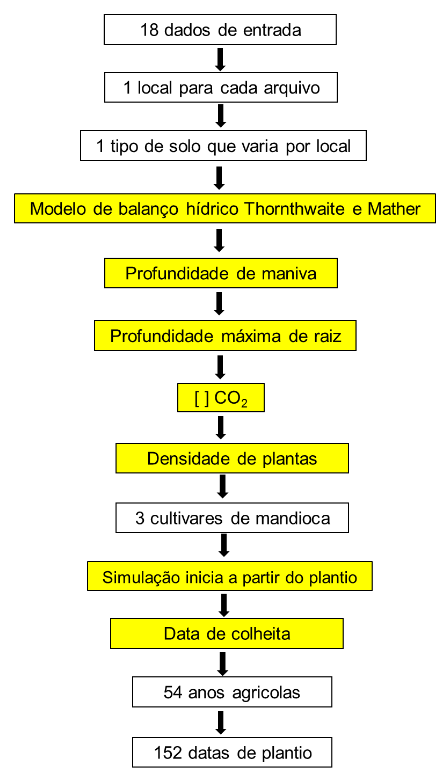
\includegraphics[width=0.4\textwidth]{imagens/SimanihotFlux}
            		\caption{Fluxograma do caso de uso 1.}
            		\label{fig:SimanihotFlux}}
            	\end{figure}
                \bigskip

                %caso 2_______________________________________________________________________

                \hrule \bigskip
            	{\bf Caso de Uso 2:}
                    Automação de simulações no modelo SoySim para simular o crescimento, desenvolvimento e produtividade de Soja para o estado do Rio Grande do sul
            	    \bigskip

            	{\bf breve descrição:}
                    Fazer simulações para 37 pontos espalhados no Rio Grande do Sul (37 arquivos de dados meteorológicos), com 120 anos de dados em cada arquivo, de 1980 a 2099, utilizando 7 datas de semeadura (01/08, 01/09, 01/10, 01/11, 01/12, 01/01 e 01/02) e 3 grupos de maturação (4.8, 5.5 e 6.0), em 2 cenários climáticos futuros. Dois conjuntos de dados com 37 arquivos de dados meteorológicos cada um. Dividindo cada um desses 37 arquivos em 3 arquivos com 45 anos de dados, pois o modelo SoySim não suporta fazer a simulação com um arquivo de dados tão extenso.
            	    \bigskip

            	{\bf Fluxo Principal:}
                	\begin{enumerate}
                		\item Inserir um arquivo de entrada para cada ponto (27\underline51 – 1960\underline2007, 27\underline51 – 2006\underline2053, 27\underline51 – 2052\underline2099, 27\underline52 – 1960\underline2007, 27\underline52 – 2006\underline2053, 27\underline52 – 2052\underline2099 e assim por diante).
                		\item Realizar as simulações para os grupos de maturação (4.8, 5.5 e 6.0).
                		\item Para cada arquivo de entrada realizar simulações que variam de 01 de agosto até 01 de fevereiro, iniciando na semeadura, de um em um mês
                		\item Modificar a densidade de população de plantas para 315.
                		\item Depois de preencher estes campos, clicar no botão \emph{run}.
                		\item Copiar os dados a partir da linha 14 a 59 do arquivo de resultado “TmpOut.txt” e armazenar todos em um só resultado filtrando itens específicos e gerar um arquivo de resultado com o mesmo.
                	\end{enumerate}

            	{\bf Fluxo Secundário:}
                	\begin{enumerate}
                		\item Reiniciar a automação alterando a automação para que a mesma não seja rodada na função de \emph{multiple years} mas sim seja rodada na função de \emph{single years}, onde cada ano precisa ser definido na interface.
                		\item Copiar a linha 35 do arquivo resultante “TmpOut.txt” e adicioná-la ao final de um arquivo de resultado único.
                	\end{enumerate}

            	{\bf Fluxo de exceção:}
                	\begin{enumerate}
                		\item No caso de encontrar algum alerta de campo preenchido incorretamente, encerrar a automação e envia o usuário para a pós condição.
                		\item Caso o modelo apresente um alerta rodando no fluxo principal o programa deve passar para o fluxo secundário
                		\item Caso o alerta seja recebido enquanto o modelo já está no fluxo secundário, passar para o ano seguinte da lista de anos da automação.
                		\item Em caso de qualquer interação do usuário durante a tarefa de automação, pausar a simulação e esperar que o usuário recomece a automação ou cancele.
                	\end{enumerate}
            	\bigskip \hrule

                %IMAGEM = fluxograma caso 2

                \bigskip
            	\begin{figure}[!htb]
            		{\centering
            		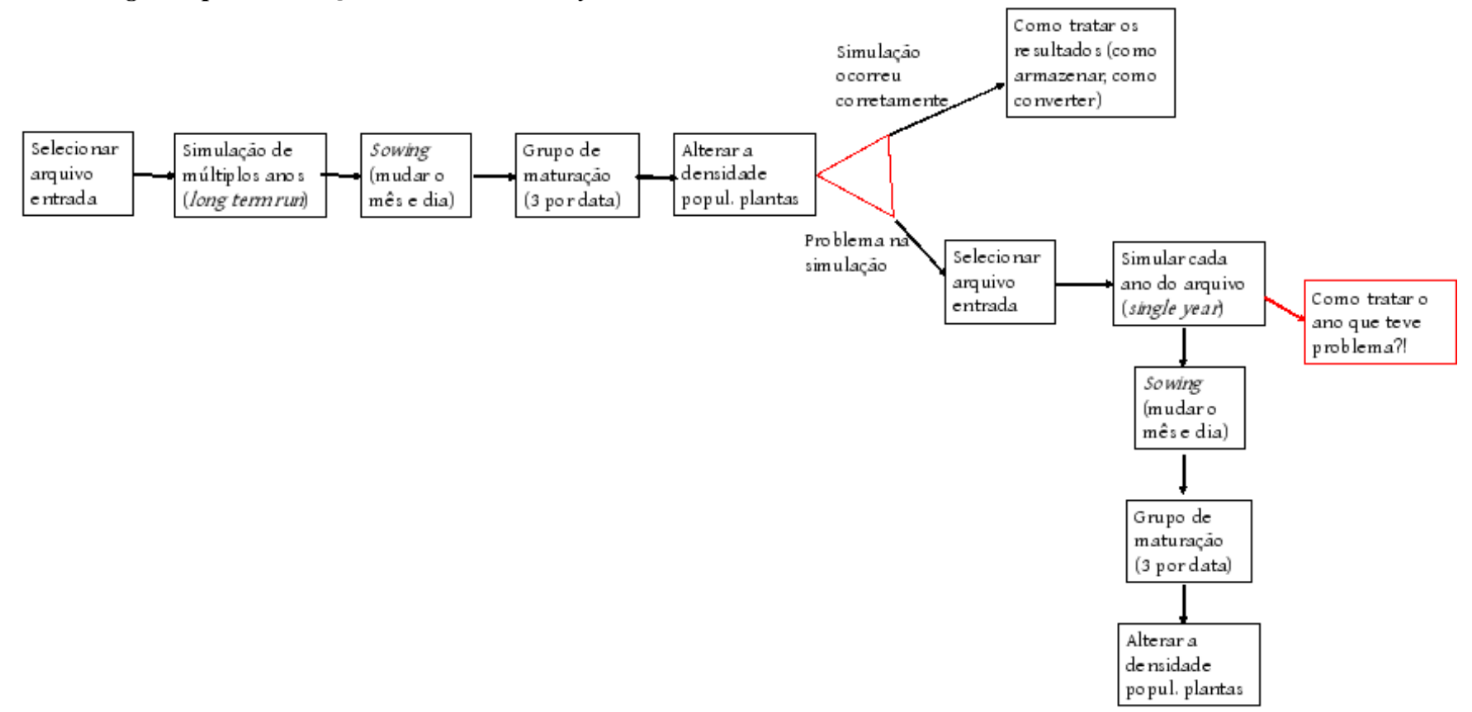
\includegraphics[width=1.0\textwidth]{imagens/SoysimFlux}
            		\caption{Fluxograma do caso de uso 2.}
            		\label{fig:SoysimFlux}}
            	\end{figure}
                \bigskip

            	%caso 3_______________________________________________________________________

                \hrule \bigskip
            	{\bf Caso de Uso 3:}
                    Automação de simulações no modelo DSSAT para gerar previsões de safra de soja para auxiliar no planejamento agrícola do Estado do Rio grande do Sul
            	    \bigskip

                {\bf breve descrição:}
                    O RS é um dos Estados brasileiros que mais sente os efeitos dos fenômenos El Nino e La Nina, e atualmente é o terceiro maior responsável pela produção de soja do País. É necessário gerar previsões de safra de soja para auxiliar no planejamento agrícola do Estado do Rio grande do Sul (RS). gerando várias simulações no modelo para diversas datas de semeadura.
                    \bigskip

            	{\bf Fluxo Principal:}
                	\begin{enumerate}
                		\item  Abrir o DSSAT, esperar carregar e clicar em \emph{Crop Management Data}. A partir dessa ação, o programa XBuild inicializará, e o usuário deve então clicar em New (para começar a criar um experimento).
                		\item  Criar um nome inexistente para o experimento. \emph{Institute Code} (SM para UFSM), \emph{Site Code} (RS se for dentro do RS), \emph{Year} (2013), \emph{Experiment Number} (99 datas de semeadura), por exemplo. Lembrando que o usuário é livre para escolher a forma de preencher as lacunas dessa etapa do experimento, de uma forma que o torne auto-explicativo. No campo \emph{Crop} (selecione \emph{Soybean}). As demais lacunas podem ser preenchidas com -99.
                		\item Nessa etapa o usuário clica em \emph{Environment} e depois em \emph{Fields}. Aqui basicamente deve ser informado qual a série meteorológica o experimento vai utilizar, se existe algum tipo de drenagem e as características do solo daquela região. Ao rodar o modelo para outro local, o usuário deve adicionar mais um “\emph{level}” e repetir o preenchimento com a série meteorológica e as características do segundo local, e assim sucessivamente.
                		\item O usuário clica em \emph{Management} e seleciona \emph{Cultivars}, a tela sera redirecionada para uma seção onde deve ser selecionada a cultivar ou as cultivares que serão utilizadas nas rodadas do modelo. Lembrando que essas já devem estar devidamente calibradas pois caso contrário, o nome da cultivar não aparecera na lista de seleção.
                		\item Inserção da data ou datas de semeadura, data de emergência, o método utilizado, a forma de distribuição das sementes, a densidade de sementes na semeadura, a densidade de plantas na emergência, o espaçamento entre linhas adotado, a direção das linhas em relação ao Norte e a profundidade de semeadura utilizada para um ou vários experimentos. Lembrando que se o experimento possui alguma característica diferente, esse deve ser inserido como um Novo \emph{Level}.
                		\item Determinar a data que o modelo vai começar a simulação do balanço hídrico ou de nutrientes no solo. É aconselhado começar o balanço hídrico no solo entre 20 e 30 dias antes da data de semeadura, buscando uma simulação mais precisa das condições do solo na hora da semeadura.
                		\item Selecionar os balanços que gostaria que o modelo realizasse em cada experimento. Aqui pode ser ativado ou não o balanço hídrico, de nitrogênio entre outras. Esses detalhes podem aumentar o desempenho das simulações.
                		\item Decidir os métodos que serão utilizados nos balanços que foram selecionados no passo anterior. Se o balanço hídrico foi selecionado, aqui o usuário deve selecionar o método que o modelo deve utilizar para as rodadas em cada experimento. Essa regra também vale para os outros balanços que o usuário deseja que o modelo realize.
                		\item Caso o usuário tenha dados mais específicos ou tenha utilizado irrigação em algum dos experimentos que deseja simular, essa é a etapa em que vai inserir as características do manejo utilizado.
                		\item Seleciona as informações que serão exibidas no final das rodadas como: Crescimento de massa seca diária, balanço hídrico....entre outros.
                		\item Caracterizar cada experimento, identificando cada experimento que vai utilizar a primeira estação meteorológica por exemplo, ou o solo número 1 entre outras informações.
                		\item Após realizar essas etapas o usuário deve clicar no botão \emph{Refresh}, que irá atualizar as novas informações e posteriormente pode abrir o programa DSSAT e começar a rodar os experimentos cadastrados.
                	\end{enumerate}

                {\bf Fluxo Secundário:}
                	\begin{enumerate}
                		\item Nenhum
                	\end{enumerate}

                {\bf Fluxo de exceção:}
                	\begin{enumerate}
                		\item No caso de encontrar algum alerta conhecido do modelo tais como alerta de temperatura máxima menor que a mínima, encerrar a automação e envia o usuário para a pós condição.
                		\item Em caso de qualquer interação do usuário durante a tarefa de automação, pausar a simulação e esperar que o usuário recomece a automação ou cancele.
                	\end{enumerate}
            	\bigskip \hrule \bigskip

        	\subsection{Analise dos casos de uso em outras ferramentas de automação}

            	Após a coleta dos casos de uso, foi analisado como outras ferramentas existentes atualmente, modelam os problemas observados nos casos de uso coletados, objetivando compreender como e sob quais condições, estas ferramentas conseguem solucionar os casos de uso.

                Dentre as ferramentas escolhidas, foram selecionados três programas de automação de interfaces gráficas capazes de solucionar os casos de uso. Os três programas escolhidos foram descritos na revisão bibliográfica deste projeto, sendo estes, UiPath, Sikuli e Autoit.

            	Como forma de avaliação adicional do quanto estas ferramentas se mostram acessíveis aos domínios de conhecimento do usuário, foi proposto a um dos atores dos casos de uso, que este tentasse utilizar as mesmas ferramentas de automação descritas na revisão literária, para resolver seu caso de uso. Descrevendo a experiência de forma objetiva, em prós e contras, analisando se foi obtido sucesso ou não e onde os problemas responsáveis pelas falhas se originaram, caso encontrado algum.
            	\bigskip

        		{\centering
                    \begin{tabular}{ | m{15.6cm} | }
            		    \hline \\
                		{\bf UiPath:} \\ \\
                		{\bf Prós:}
                            O programa permite virtualmente a realização de qualquer tarefa por meio da construção de um fluxograma, com diversos elementos, vários deles autoexplicativos, tais como as regras de interação de clique e digitação na interface dos modelos matemáticos. Fornece lógica suficiente para as repetições e iterações necessárias nos casos de uso, também permite mover ou renomear arquivos para que as rodadas não se sobrescrevam no caso 2. \\ \\
                		{\bf Contras:}
                            O programa é muito complexo, fator especialmente observado ao tentar modelar regras para o tratamento de erros no caso 1 e 2, contem muitas opções, elementos carregados e complexos e poucas funções realmente genéricas. Em outro exemplo de complexidade, alguns elementos envolvem expressões VisualBasic.
                            Depende da chamada de métodos externos ao programa para tarefas não contempladas pelos elementos de fluxograma, fator necessário no \emph{parsing} de valores em arquivos necessários para o caso 2, o que envolve métodos tradicionais de automação, com linguagens de programação convencionais, podendo recorrer inclusive ao \emph{powershell}. \\ \\
                		\hline

                        \hline \\
                        {\bf Sikuli:} \\ \\
                		{\bf Prós:}
                            O programa é fácil de entender com elementos autoexplicativos e não muito complexos, é capaz de realizar as tarefas básicas tais como interagir com a interface do modelo e esperar por eventos. \\ \\
                		{\bf Contras:}
                            Para os casos de uso, os elementos visuais presentes não são suficientes e não contemplam repetições, trabalhar com arquivos, tratar erros, dentre outros, tornando necessário que o usuários recorra a linguagem Python para realizar a automação. \\ \\
            		    \hline
                    \end{tabular} \\

                    \begin{tabular}{ | m{15.6cm} | }
                		\hline \\
                		{\bf AutoIt} \\ \\
                		{\bf Prós:}
                            Novamente um programa capaz de realizar virtualmente qualquer tarefa. Apesar de sua abordagem bastante tradicional de programação em texto, possui uma biblioteca bem ampla de funcionalidades.\\ \\
                		{\bf Contras:}
                            O programa é totalmente dependente de linguagem \emph{script} tipo BASIC própria, sem nenhum elemento visual ou autoexplicativo. A automação se torna um desafio possivelmente tão grande quanto o problema original, já que o usuário precisa conhecer com certa profundidade a linguagem, o programa e as bibliotecas do AutoIt. \\ \\                		\hline
        	       \end{tabular}
                }

            	\bigskip
            	Analise do caso de uso 2 realizada pelo autor de forma direta nos 3 programas de automação sugeridos sem intervenção de terceiros ou qualquer pessoa do domínio da área:
            	\bigskip

            	{\centering
                    \begin{tabular}{ | m{15.6cm} | }
                		\hline \\
                		{\bf Caso de uso 2 Analisado pelo ator} \\
                		\begin{center}
                            Automação de simulações no modelo SoySim para simular o crescimento, desenvolvimento e produtividade de Soja para o estado do Rio Grande do sul.
                        \end{center}
                		\\ \hline \hline \\
            	        {\bf UiPath:} \\ \\
                		{\bf Prós:}
                            Conseguiu fazer com que o software rodasse o SoySim para \emph{SingleYear} e  \emph{LongTermRun}. Uma rodada sozinha. \\ \\
                		{\bf Contras:}
                            Não conseguiu inserir um \emph{loop} para que múltiplas rodadas fossem feitas, também não conseguiu fazer com que o programa mudasse os arquivos de entrada automaticamente. Além disso, não conseguiu fazer com que o programa entendesse a janela de erro do SoySim. \\ \\
            		    \hline
                    \end{tabular} \\

                    \begin{tabular}{ | m{15.6cm} | }
                        \hline \\
                		{\bf Sikuli:} \\ \\
                		{\bf Prós:}
                            consegui montar o scrit que é no mesmo formato do UiPath (visual).  \\ \\
                		{\bf Contras:}
                            Na hora de rodar, o programa apresentou um erro que o ator não consegue interpretar, erro apresentado na figura \ref{fig:erroSikuli}. Desistiu da ferramenta devido ao erro. \\ \\
                		\hline \hline \\
                		{\bf AutoIt} \\ \\
                            O ator não conseguiu compreender minimamente como a ferramenta funciona, foi capaz de perceber que o programa usa código textual para automatizar as tarefas mas por não ter profundo contato com linguagens de programação ou BASIC, não foi capaz de encontrar uma solução intuitivamente ou em tempo hábil no manual do programa. Desistiu da ferramenta devido à dificuldade. \\ \\
            	       \hline
            	   \end{tabular}
                }

            	\begin{figure}[!htb]
            		{\centering
            		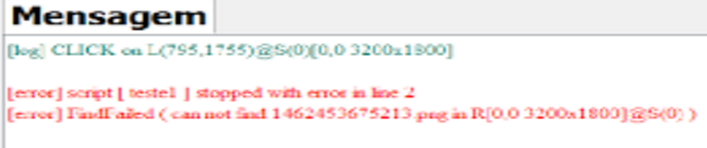
\includegraphics[width=1.0\textwidth]{imagens/sikuli_error}
            		\caption{Erro obtido pelo autor no programa Sikuli.}
            		\label{fig:erroSikuli}}
            	\end{figure}

                Observando as informações obtidas ao analisar os casos de uso com outras ferramentas de automação, foram encontrados alguns pontos relevantes para a Proposta do projeto.

                \begin{enumerate}
                   \item Linguagens de programação tradicional não contribuem para os atores solucionarem seus problemas e inclusive dificultam a obtenção de uma solução em alguns casos.

                   \item Apesar de possibilitar a solução, teoricamente, de qualquer problema inclusive fora da automação de interfaces gráficas, linguagens de programação tradicional são desnecessariamente complexas para os atores e inclusive, para o problema deste projeto, aumentaram as duvidas dos atores e problemas que eles precisavam considerar durante a obtenção de uma solução, tal como a validade sintática de suas soluções assim como coleta de informações em outras fontes com relação a vocábulos e semântica da linguagem.

                   \item Os momentos em que os atores mais se beneficiaram das ferramentas analisadas foi quando as mesmas ofereceram, componentes sucintos e autoexplicativos, ou seja, que descreviam o que fazem, como usá-los e como não usá-los.

                   \item O segundo momento em que os atores mais se beneficiaram das ferramentas analisadas foi quando os componentes oferecidos interagiam com os atores, impedindo maneiras incorretas de seu uso ou explicitando o uso correto por meio de diversas simbologias tais como o encaixe perfeito entre os elementos, dentre outros.

                   \item O elemento-chave para os atores residiu na capacidade ou não da ferramenta em explicar o que se pode fazer ou não, tomando para sí algumas tarefas que exigem atenção, como a analise em algum nível da validade da solução.
                \end{enumerate}

            \subsection{Coleta dos requisitos funcionais}

                Com base nas informações obtidas durante a analise prévia do problema, dos casos de uso, analise de ferramentas existentes, assim como discussão com os atores envolvidos, surgiram ideias de funcionalidades, das quais foram selecionados alguns requisitos funcionais mínimos para se chegar ao objetivo deste projeto assim como a solução dos problemas principais nos casos de uso.

                \begin{enumerate}

            		\item Deve ser possível executar, salvar ou carregar automações construídas pelo ator de forma que se possa reutilizar estas automações, construídas anteriormente no programa. Também é preciso que seja possível descartar a automação.

            		\item Dois elementos, um capaz de executar a ação de clicar uma vez em uma área da tela e outro capaz de executar a ação de clicar duas vezes em uma área da tela; o ator deve ser capaz de escolher a área da tela para cada instância do elemento e o elemento deve representar a área onde irá realizar a ação.

            		\item Um elemento capaz de esperar por uma alteração na tela ou evento que indique que a automatização pode prosseguir para as próximas tarefas definidas pelo ator.

                   \item Um elemento capaz de digitar textos nos campos do programa a ser automatizado, como se fosse o usuário digitando.

                   \item Elementos complementares que consigam expressar a lógica, condições, repetições ações e valores tais como números e textos.

                   \item Um elemento capaz de ler ou gravar um arquivo de texto de forma que se possa alterar o texto lido ou que se possa apenas copiar o arquivo para outro lugar, podendo mudar o nome.

                   \item Um elemento que permita tomar decisões que alterem o fluxo de automação.

                   \item Uma forma de pausar ou continuar a simulação.

            	\end{enumerate}

        \section{Modelagem}

            Para que um software possa automatizar outro software com interface gráfica, é necessário que o software que realiza a automação possa enviar informação para o software a ser automatizado assim como sua interface gráfica. Analogamente, é preciso que o software automatizador possa receber informação do software a ser automatizado.

            Possibilitar que o software automatizador envie e receba do software a ser automatizado,  envolve estabelecer quais são as possíveis entradas e saídas do software a ser automatizado, sabendo que este desconhece a existência do automatizador, para em seguida definirmos as entradas e saídas do software automatizador, estabelecendo assim, nossa interface de comunicação.

            Após conhecermos as entradas e saídas do software a ser automatizado serão modeladas as entradas e saídas do software automatizador, visando estabelecer uma interface com o software que queremos automatizar. Ao mesmo tempo, serão modelados os componentes internos que dão ao software automatizador, as condições necessárias para realizar as funcionalidades concebidas durante a coleta de requisitos.

            A entrada e saída precisará também ser modelada considerando como o ator ou usuário irá interagir com o software automatizador para que este realize a automação necessária. A esquematização da interação entre o software automatizador, o usuário e o software a ser automatizado, pode ser observado na figura \ref{fig:generalIO}.

            \begin{figure}[!htb]
                {\centering
                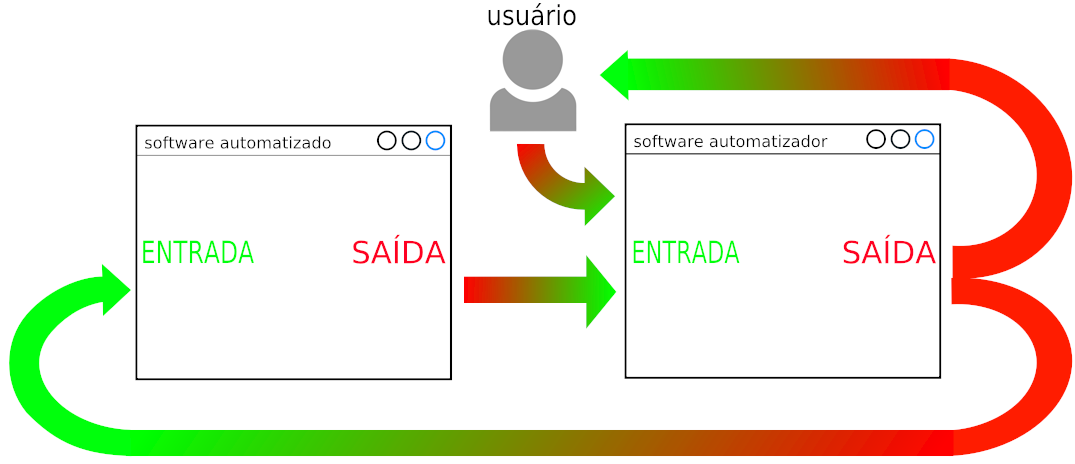
\includegraphics[width=1.0\textwidth]{imagens/generalIO}
                \caption{Descrição da interação entre o software automatizador e o software a ser automatizado, incluíndo o usuário ou ator que irá utilizar o automatizador.}
                \label{fig:generalIO}}
            \end{figure}

            \subsection{Entradas e saídas do software a ser automatizado}

                Para definir as entradas e saídas do software a ser automatizado\footnote{Nesta seção, iremos nos referir a eles como “software a ser automatizado” ou apenas software.}, foi utilizado os modelos matemáticos de simulação de culturas agrícolas escolhidos para serem automatizados neste projeto.

                Considerou-se quais eram os elementos com os quais se podia interagir, formas de interação e resultados observados. A figura \ref{fig:modelIO} descreve as entradas e saídas observadas durante a análise dos softwares, sua natureza e componentes de destino ou origem. Essas entradas e saídas foram discretizadas em dois tipos de entrada e dois tipos de saída:

                \begin{itemize}
                    \item entradas:
                        \subitem {\bf ações}: Interações que resultam em alguma saída do software, seja eventos ou dados.
                        \subitem {\bf dados}: Interações que fornecem dados ou valores, precedidos de uma ação, podendo resultar em um evento.
                    \item saídas:
                        \subitem {\bf eventos}: Eventos ou respostas que buscam informar o usuário de alguma condição atingida no software, decorrente de alguma entrada, seja ação ou dado, podem esperar a interação do usuário.
                        \subitem {\bf dados}: Dados e novas informações produzidas pelo software, produto final esperado pelo usuário, decorrente de algum evento.
                \end{itemize}

                \begin{figure}[!htb]
                    {\centering
                    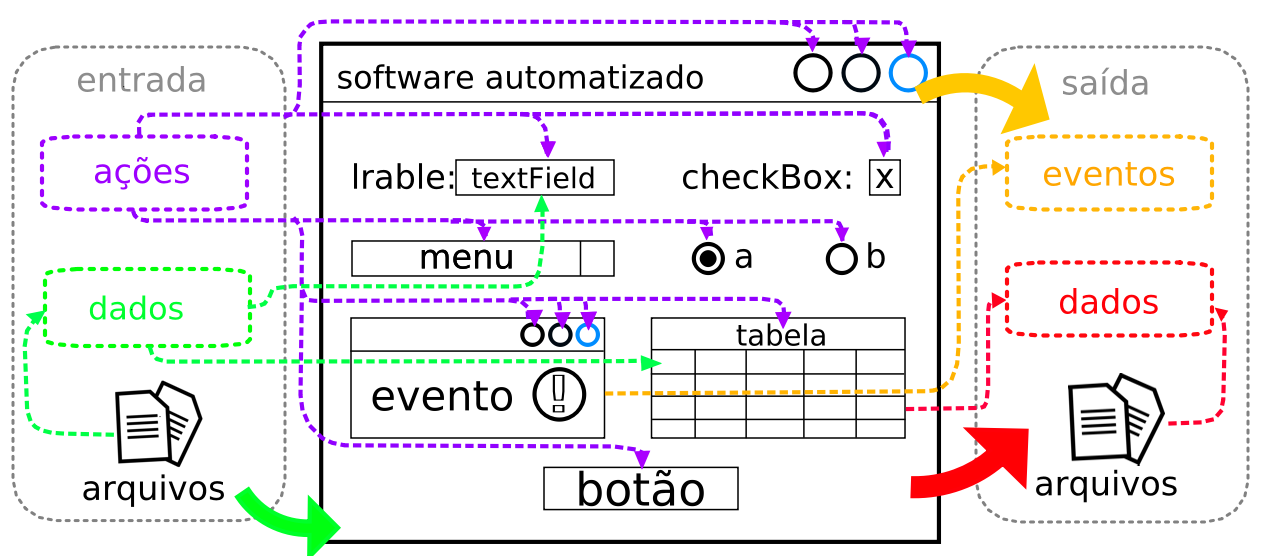
\includegraphics[width=1.0\textwidth]{imagens/modelIO}
                    \caption{Descrição das entradas e saídas do software a ser automatizado, as grandes cetas reqpresentam o software como um todo, como destino ou origem, a verde mostra que é possível inserir arquivos no software, a vermelha, que é possível obter arquivos do software, e a laranja indica que, não somente mensagens, mas qualquer componente do software pode representar um evento, mudando de estado.}
                    \label{fig:modelIO}}
                \end{figure}

                Como é possível observar na figura\ref{fig:modelIO}, as ações correspondem a entradas que podem resultar em alguma saída, logo, podem produzir eventos ou dados como saída, podendo inclusive produzir ambos. As ações são consideradas entradas que ativam elementos ou funções do software.

                Os dados quando considerados como entrada, podem ser inseridos de duas formas: após alguma ação, que indica que o dado pode ser inserido no componente foco da ação, como por exemplo em um \emph{textfield}, onde pode se inserir valores tal como números, texto ou a localização de arquivos, ou ainda podem ser inseridos automaticamente após alguma ação, caso o programa sempre procure por arquivos em algum local específico quando iniciado, onde a ação é a execução do software. Inserir dados resulta em  evento, como por exemplo, mudança de estado do componente que recebe os dados ou uma mensagem.

                Quando consideramos os eventos de saída, estes resultam, de alguma entrada. Os eventos procuram informar o usuário de alguma condição satisfeita por uma entrada, como por exemplo, sucesso na inserção de um arquivo, ou de algum problema que deve ser observado, como por exemplo, algum campo preenchido incorretamente, ou que por exemplo, um elemento recebeu um evento e obteve foco, esperando pela inserção de dados.

                Finalmente, considerando os dados de saída, podem ser observados duas formas: dados que são apresentados em componentes da interface gráfica, no caso dos softwares observados, podemos citar componentes como tabelas, gráficos e arquivos, que no caso dos softwares observados, são arquivos de texto. Os dados de saída são gerados por ações, quando gerados automaticamente, se deve ao fato de que o modelo tem a capacidade de acessar e carregar automaticamente resultados produzidos em algum momento no passado, estes dados são gerados após a inicialização do software ou seleção de simulação específica.

                De forma resumida, do ponto de vista dos softwares observados, podemos observar que todas as saídas resultam de alguma entrada e inclusive a entrada de dados depende de alguma ação prévia, Incluindo aqui o ato de iniciar o software. Analogamente, podemos deduzir que toda entrada resultará em pelo menos uma saída, seja esta um evento ou um dado.

                Comportamentos diferentes foram considerados exceções, podendo resultar do fato de que o software parou de responder (receber entradas ou produzir saídas), ou a entrada fornecida resultou em saídas não esperadas pelo usuário.

            \subsection{Modelagem do software Automatizador}

                Feitas as observações de quais são as entradas e saídas do software que será automatizado e considerando que a automatização depende da interação entre ambos, é possível deduzir que a saída do automatizador\footnote{ Nos referiremos ao software automatizador como “automatizador” ou “software automatizador”.} precisa conter elementos do mesmo tipo que a entrada do software a ser automatizado, direcionada a entrada do software a ser automatizado.

                Analogamente, podemos deduzir que a entrada do automatizador precisa conter elementos do mesmo tipo que a saída do software a ser automatizado. Como o software automatizado desconhece a existência do automatizador, o automatizador precisa procurar e filtrar, quando necessário, saídas do tipo que o software a ser automatizado gera.

                Além das entradas e saídas necessárias para estabelecer uma interface com o software automatizado, o automatizador também necessita estabelecer uma interface com o usuário.

                Considerando o usuário e o software a ser automatizado, as entradas e saídas do automatizador foram discretizadas em três tipos de entrada e três tipos de saída:

                \begin{itemize}
                    \item entradas:
                        \subitem {\bf ações}: Interações vindas do usuário, que podem resultar em alguma saída do automatizador, seja eventos dados ou ações.
                        \subitem {\bf eventos}: Uma das saída do software a ser automatizado, procurados quando necessário durante a automatização.
                        \subitem {\bf dados}: Quando inseridas pelo usuário, interações que fornecem dados ou valores para o automatizador realizar a automação, ou então, uma das saídas do software automatizado, procurados quando necessário durante a automatização. Podem resultar em algum evento no automatizador.
                    \item saídas:
                        \subitem {\bf ações}: Ações geradas pelo automatizador durante a automação, destinadas a entrada de ações do software a ser automatizado.
                        \subitem {\bf eventos}: Eventos ou respostas que buscam informar o usuário de alguma condição atingida no automatizador, decorrente de alguma entrada do usuário, seja ação ou dados, podem necessitar a interação do usuário.
                        \subitem {\bf dados}: Podem tanto ser dados produzidos pelo automatizador durante a automação, destinados a entrada de dados do software a ser automatizado, como dados produzidos por alguma ação do usuário sobre o automatizador, que não são destinados ao software a ser automatizado.
                \end{itemize}

                \begin{figure}[!htb]
                    {\centering
                    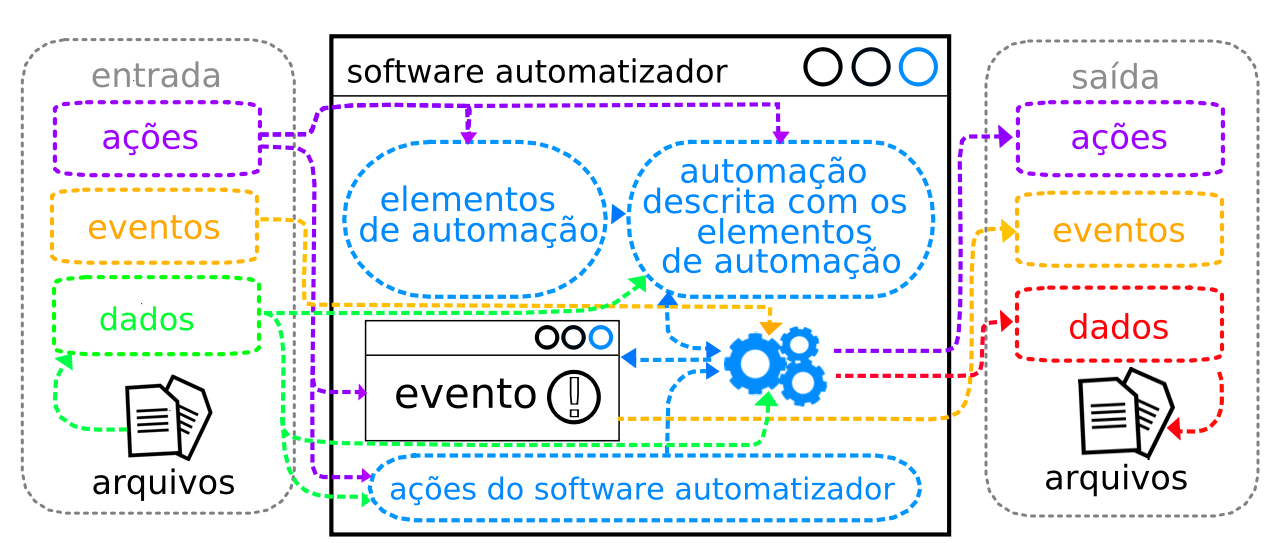
\includegraphics[width=1.0\textwidth]{imagens/automatIO}
                    \caption{Descrição das entradas e saídas do automatizador, assim como da definição dos seus componentes internos. As engrenagens simbolizam os componentes de controle do automatizador.}
                    \label{fig:automatIO}}
                \end{figure}

                Podemos observar na figura \ref{fig:automatIO}, que a entrada de ações por ser realizada pelo usuário, é destinada a componentes do automatizador considerados acessíveis ao usuário, podem ser necessários nos eventos gerados pelo automatizador para tomar decisões, nos elementos de automação para selecioná-los para montar a descrição da automação, assim como na descrição da automação para alterá-la, ocorrem também nas ações do software automatizador, quando o usuário, por exemplo, decide executar a automação. Geram alguma das saídas previstas no automatizador

                A entrada de eventos ocorre seletivamente durante a automação, onde o software a ser automatizado é observado de acordo com regras definidas na descrição da automação em buscas de condições descritas pelo usuário na descrição da automação. Quando relevantes para a automação. Poderão resultar em alguma saída do automatizador, a depender da satisfação ou não da condição.

                Já a entrada de dados pode vir tanto do usuário como do software a ser automatizado. Quando do usuário, são destinados a descrição da automação ou eventos, caso contrário, são buscados seletivamente durante a automação, no software a ser automatizado, dependendo de como a automação foi descrita pelo usuário. Podem produzir eventos quando inseridos pelo usuário que podem necessitar atenção do mesmo. Também alteram ou geram saídas destinadas ao software a ser automatizado, quando obtidos do software automatizado.

                Na saída do automatizador as ações são produtos da execução da automação descrita com os elementos de automação, destinadas ao software a ser automatizado. Podem produzir eventos ou dados como saída no software automatizado que são do interesse do automatizador.

                Os eventos, quando considerados como saída, são mensagens do automatizador destinadas ao usuário. São produtos de alguma entrada e indicam a satisfação ou não de alguma condição que necessita atenção, portanto, podendo necessitar a inserção de dados ou realização de alguma ação por parte do usuário.

                Já a saída de dados pode ser tanto oriunda da execução da descrição da automação, destinadas ao software automatizador, como de ações realizadas pelo usuário, que não visam interagir com o software a ser automatizado, por exemplo, salvar a automação em um arquivo.

                \subsection {Componentes do  software automatizador}

                    Ainda podemos observar na figura \ref{fig:automatIO}, quatro componentes importantes para o automatizador, que permitem a realização das funcionalidades descritas nos requisitos.

                    Os elementos de automação são a coleção léxica da linguagem de automação, lexemas, unidades mínimas dotadas de significado lexical, componentes simbólicos com significado que descrevem alguma operação, condição, regra, elemento ou informação na automação. Estes elementos, por sua vez, são arranjados e conectados em ordem específica definida por suas propriedades, para formar a automação descrita com os elementos de automação.

                    Temos também um conjunto especial de ações do software automatizador que definem as ações do automatizador, o que deve ser feito com a automação descrita com os elementos de automação. Funcionalidades que dependem deste conjunto de componentes são, por exemplo, a capacidade de salvar automações ou ainda de executar a automação.

                    Todos os três elementos anteriores estão diretamente acessíveis ao usuário devido ao fato de que o usuário interage com eles, entretanto, apenas estes elementos sozinhos não são capazes de realizar e coordenar adequadamente suas funções e interações entre si, muito menos delegar os resultados destas funções e interações aos seus destinatários, seja este o software automatizado ou o usuário.

                    Quem faz este papel são os elementos de controle do automatizador que não estão diretamente acessíveis ao usuário, porém respondem as interações do mesmo com os outros elementos descritos, realizando as tarefas requisitadas pelos componentes assim como o envio e recebimento de informações entre eles pertinentes para as tarefas requisitadas, com o objetivo de concretizar as funcionalidades definidas na coleta de requisitos assim como o objetivo final, automatizar o software a ser automatizado.

                    São descritos na figura \ref{fig:automatIO} como engrenagens e são os componentes responsáveis por controlar o automatizador, sendo responsáveis por diversas tarefas dentro do software automatizador, dentre elas:

                    \begin{itemize}
                        \item Carregamento de todos os elementos do automatizador com as propriedades e estado necessários na inicialização do automatizador.
                        \item intercomunicação entre todos os componentes quando requisitados por algum componente por intermédio do usuário.
                        \item realização das tarefas e do processamento requisitados pelos componentes a depender da funcionalidade que eles representam e dado que eles contem.
                        \item Apresentação de eventos e transmissão de informações dos mesmos para os outros componentes ou vice-versa.
                        \item Coordenador na tarefa de utilização dos elementos de automação pelo usuário para serem usados na descrição da automação.
                        \item realização das ações do software automatizador como executar, salvar, excluir ou carregar uma automatização salva.
                        \item Criação e delegação das informações de saída produzidas pelas tarefas descritas nessa lista.
                    \end{itemize}

        \section {Desenvolvimento do software}

            Com o software modelado é preciso criar os componentes idealizados, no desenvolvimento do software serão analisadas soluções para estes componentes, procurando as melhores soluções viáveis para satisfazer o objetivo deste projeto e requisitos elencados, embasando-se em observações feitas durante a concepção e modelagem para posteriormente, codificar o software, onde alguns trechos relevantes da codificação serão apresentadas e discutidas.

            \subsection {Interação com o software a ser automatizado}

                O primeiro problema observado durante a modelagem foi a necessidade de de interagir com o software automatizado, sendo que este não está ciente do automatizador. Foi identificado que o automatizador necessita enviar ações e dados para o software a ser automatizado, assim como precisa ser capaz de ler eventos e dados do software a ser automatizado.

                Soluções observadas em outros softwares de automação testados durante o estudo dos casos de uso e revisão literária deste projeto envolviam duas formas de interação com o software a ser automatizado, utilização de APIs específicas do sistema, onde um exemplo de software analisado que utiliza este método como parte de suas funcionalidades, é o AutoIt, ou ainda, o método de captura e execução, método utilizado por outro software observado na análise dos casos de uso, o Sikuli ou Sikulix. A utilização de uma APIs ainda pode ser dividida em duas abordagens em sistemas Windows, o método baseado em \emph{windows handles} (em sistemas UNIX, componentes similares seriam \emph{file descriptors}) e o método baseado em \emph{Windows Controls}.

                \emph{Handles} são identificadores únicos que fornecem encapsulamento abstrato e opaco para recursos internos do software que neste caso queremos automatizar, eles podem ser utilizados para identificar qualquer recurso dentro do software, indo além dos recursos observados apenas na interface, podem ser identificadores da janela do software, de um botão ou até mesmo, componentes internos como listas, \emph{threads} dentre outras estruturas e recursos utilizadas pelo software. Os \emph{windows handles} são uma abstração particular dos recursos de um software em sistemas operacionais Windows. Em sistemas operacionais UNIX, uma abstração similar são \emph{file descriptors}.

                \emph{Windows controls} por sua vez são também abstrações em sistemas Windows, são janelas filhos que o software usa em conjunto com outra janela que tornam possível a interação do usuário com o software. Em sistemas UNIX não existe uma abordagem padrão, já que alguns componentes de \emph{frameworks} mais modernos podem ser acessíveis apenas na aplicação cliente e não no servidor X, isso quando consideramos que o servidor de vídeo em uso é o servidor X. Um exemplo de \emph{framework} que permite acessar estes componentes em aplicações GTK é o ATK.

                O método de captura e execução é baseado em captura e análise de imagens obtidas da tela do computador com o intuito de localizar elementos para posteriormente indicar uma interação padrão do usuário a ser realizada no elemento localizado, como ações de mouse e teclado. Outra abordagem ainda seria gravar a interação do usuário como movimentação do mouse e locais clicados e digitados. A abordagem é a mesma independente do sistema operacional.

                Na tabela a seguir serão analisados os pontos positivos e negativos das três abordagens.

                \bigskip
                {\centering
                \begin{tabularx}{\textwidth}{|*{1}{>{\centering\arraybackslash}X}|}
                    \hline
                    \emph{Windows handles} \\
                    \hline
                    {\bf contras:} \\
                    \begin{itemize}
                        \item Permitem um nível bastante refinado de automação e em alguns casos permitem alterar profundamente o comportamento do programa ao mudar o comportamento de componentes e inclusive o estado das informações internas do mesmo.
                        \item É mais flexível e menos dependente de padrões que o método \emph{Windows controls}. Também oferece acesso a mais recurso e propriedades do software que o método \emph{Windows controls}.
                    \end{itemize}
                    \\ {\bf contras:} \\
                    \begin{itemize}
                        \item A utilização em geral só é pratica em aplicações que o usuário conheça internamente o funcionamento, sendo relevante fazer um uso cauteloso já que \emph{handles} são intencionalmente abstratos. \emph{Handles} variam de seção para seção do programa e podem ser descartados durante a existência do programa ou simplesmente não representarem mais o mesmo elemento.
                    \end{itemize}
                    \\ \hline
                \end{tabularx}

                \begin{tabularx}{\textwidth}{|*{1}{>{\centering\arraybackslash}X}|}
                    \hline
                    \emph{Windows controls} \\
                    \hline
                    {\bf Prós:} \\
                    \begin{itemize}
                        \item Não depende da visibilidade dos \emph{controls}. \emph{Controls} que não estejam visíveis também estão ao alcance da ferramenta de automação já que a mesma tem acesso a todas as propriedades do programa.
                        \item É possível alterar o comportamento do programa já que é possível definir qualquer estado possível para um \emph{control} em específico.
                        \item A interação do automatizador é mais próxima do contexto interno do programa, enviando, por exemplo, eventos diretamente para os \emph{listeners} em botões, isso garante maior exatidão no comportamento o que é mais relevante nos casos em que se busca testar o softwares.
                        \item por não exigir muito processamento extra, analise complexa de dados e não depender da resposta da interface, é relativamente rápido.
                        \item é uma abordagem mais estável que o método baseado em \emph{windows handles} já que os \emph{controls} são mais previsíveis e padronizados.
                        \item Permite um grande reaproveitamento e reutilização em condições diversas se comparado ao método baseado em captura e execução.
                    \end{itemize}
                    \\ {\bf contras:} \\
                    \begin{itemize}
                        \item É limitado a \emph{controls} conhecidos pelo software e API automatizadora, exigindo um mapeamento de componentes customizados que diferem dos componentes tradicionais conhecidos pela API. Num exemplo, o software automatizador AutoIt apenas trabalha com os \emph{controls} padronizados da Microsoft \footnote{esta informação pode ser encontrada na documentação do software AutoIt; https://www.autoitscript.com/autoit3/docs/intro/controls.htm}.
                        \item Ainda exige um conhecimento relativo do comportamento do software a ser automatizado por parte do usuário, quais são os estados dos \emph{controls} e qual é o significado dos estados do mesmo.
                        \item Da mesma forma que no método baseado em \emph{Windows handles}, alterar livremente as propriedades dos \emph{controls} do software que se quer automatizar é perigoso já que pode levar a estados e condições inconsistentes dentro do software a ser automatizado, já que é possível definir qualquer estado possível para o \emph{control} manipulado.
                    \end{itemize}
                    \\ \hline
                \end{tabularx}

                \begin{tabularx}{\textwidth}{|*{1}{>{\centering\arraybackslash}X}|}
                    \hline
                    captura e execução \\
                    \hline
                    {\bf prós:} \\
                    \begin{itemize}
                        \item Não exige conhecimentos complexos de computação para utilização pelo usuário como compreensão de abstrações em nível de \emph{frameworks} e APIs, como \emph{handles} ou \emph{controls} e como podem ser úteis em automação.
                        \item é de uso consideravelmente rápido para o usuário, pois não é preciso analisar tabelas ou listas de componentes em busca dos \emph{handles} ou \emph{controls} corretos.
                        \item pode ser usado em quaisquer condições, inclusive programas com interfaces não convencionais, contendo elementos fora do padrão, customizados.
                        \item independe do sistema operacional ou tecnologia da interface, pode controlar programas, páginas web, etc.
                    \end{itemize}
                    \\ {\bf contras:} \\
                    \begin{itemize}
                        \item Não é tão rápido como os outros métodos por exigir captura e analise complexa de imagens.
                        \item Não é possível elaborar um padrão formal menos abstrato para entrada de dados neste método devido ao fato de que as interfaces gráficas têm um dinamismo muito variado e complexo.
                        \item A dificuldade em estabelecer um padrão formal torna difícil reutilizar automações prontas já que o método é sensível a mudanças na interface ou no ambiente.
                        \item Mesmo em ambientes controlados, pequenas mudanças na interface do software a ser automatizado podem exigir alterações na descrição da automação.
                    \end{itemize}
                    \\ \hline
                \end{tabularx}
                }

                Considerando as análises feitas das abordagens a cima, dos requisitos elencados e observações feitas na concepção do software a abordagem de captura e execução foi adotada embasado nos seguintes pontos:

                \begin{itemize}
                    \item As outras duas abordagens, apesar de possuírem pontos positivos relevantes, beneficiam muito mais a automação de testes de softwares do que a automação que este projeto busca em softwares de simulação de culturas agrícolas, onde o acesso a propriedades e estados não previstos na interface gráfica do software não são pertinentes.

                    \item A abordagem baseada em captura e execução é a que mais se aproxima do domínio de conhecimento dos usuários dos softwares que este projeto visa automatizar, já que o mesmo pode usar a abordagem com base nos conhecimentos que já obteve do uso da interface gráfica e do software. Esta proximidade pode ser observada inclusive nos requisitos coletados, onde a discussão com os atores aborda o problema em nível de ações e interações que se encaixam na abordagem, como a utilização de teclado e mouse.

                    \item As outras abordagens recorrem a conhecimentos peculiares da computação como orientação a objetos e modelos de abstração relacionados a este assunto.

                    \item Apesar de a captura e execução ser computacionalmente mais lenta, a performance não é um componente crucial para a automatização dos softwares observados, já que apesar de ocorrer repetição, a repetição não é exaustiva como nos testes de software que busca investigar todo o comportamento do software, onde a performance do método pode ser relevante.

                    \item Oferece maior flexibilidade para o usuário, já que pode ser usado em quaisquer condições, inclusive onde outras abordagens não são viáveis.

                    \item É a abordagem que menos exige analise por por parte do usuário, já que o mesmo não precisa procurar em tabelas e lista de componentes em busca de quais componentes estão relacionados com a tarefa que visa realizar no software, como encontrar qual elemento corresponde a um botão, ou campo de texto, ou funcionalidade do software a ser automatizado, ele pode utilizar os conhecimentos que já possui a respeito do software para realizar estas decisões.

                    \item Oferece menor risco de expor para o usuário, a possibilidade de usar condições que não foram previstas pelo desenvolvedor do software que ele está automatizando.
                \end{itemize}

                Além das abordagens descritas, algumas interações do usuário mostraram permitir a utilização de métodos específicos, como por exemplo a execução do software. Onde o automatizador procuraria nas variáveis de ambiente pelo software a ser executado ou ainda realizaria uma busca em todo o sistema, ou ainda, o usuário poderia selecionas o executável.

                Uma das vantagens deste método seria a execução de aplicações que não possuem um arquivo executável acessível ao usuário. Embora pertinente para a automação destes softwares, não foi observado vantagens para os softwares que este projeto objetiva automatizar, que por se focarem em usuário de programas com interface gráfica, disponibilizam executáveis que estão ao alcance do usuário por esta via.

                Além das considerações feitas a cima, estas abordagens envolvem alguns conhecimentos formais de computação que devem ser observados pelo usuário. Nem sempre é garantido que o software está devidamente registrado nas variáveis de ambiente como é possível observar no SoySim que não possui um instalador e não insere o programa na lista de caminhos de executáveis nas variáveis de ambiente do sistema operacional.
                Alguns sistemas operacionais, por exemplo, não expõem visivelmente as extensões de arquivos, o que poderia levar a ambiguidades quando o usuário informasse o nome do software a ser procurado, por considerando a extensão não relevante ou desconhecer sua existência, já que alguns softwares dentre os presentes no caso de teste divergem na sua natureza, podendo ser arquivos executáveis do Windows ou executáveis Java.

                Outra consideração é que procurar o executável poderia se tornar uma tarefa excepcionalmente lenta caso fosse necessário vasculhar a arvore do sistema. E caso o usuário conhecesse a localização do executável, utilizar a abordagem de captura e execução seria igualmente eficiente para realizar a tarefa.

                \subsubsection {utilização da abordagem escolhida}

                Foi analisado como a abordagem de captura e execução poderia ser utilizada no software automatizador e optou-se por uma abordagem onde o usuário seleciona o elemento de automação e posteriormente define no elemento, a área sob a qual ele deve agir, com base em imagens como definição de local, é possível observar uma descrição abstrata da solução na imagem \ref{fig:actionRecord}.

                \begin{figure}[!htb]
                    {\centering
                    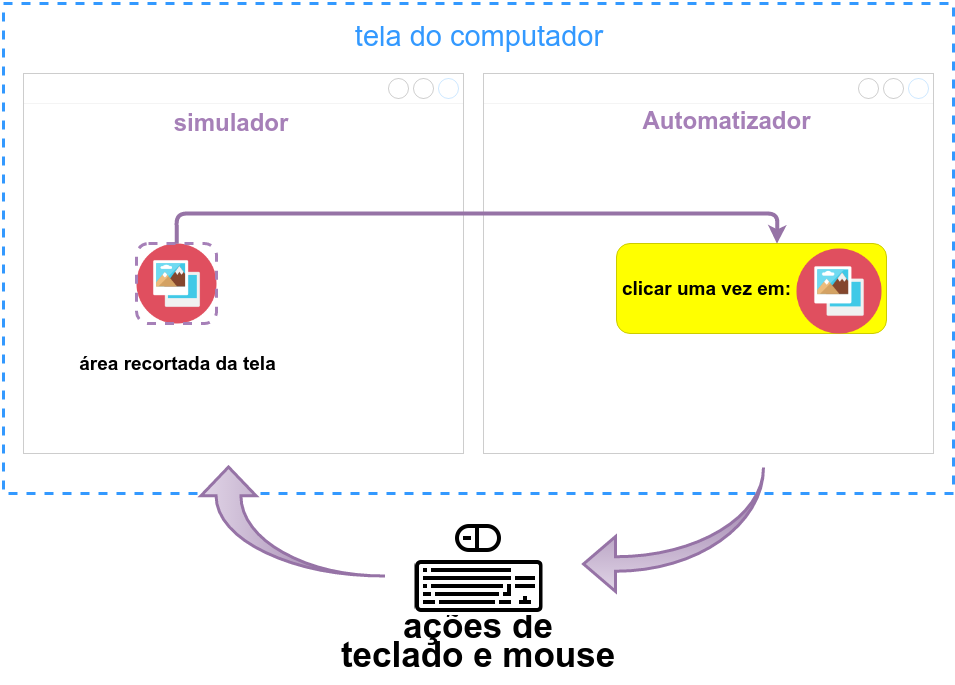
\includegraphics[width=1.0\textwidth]{imagens/actionRecord}
                    \caption{Estrutura geral da solução.}
                    \label{fig:actionRecord}}
                \end{figure}

                Nesta abordagem, as imagens capturadas do software a ser automatizado, seriam os eventos gerados pelo software a ser automatizado, quando torna a interface visível para interação, imagens estas capturadas pelo usuário. Após a localização do elemento, o automatizador pode enviar ações (controlando o dispositivo de entrada apontador, mouse), que irão gerar um evento de obtenção de foco ou ativação no elemento, objéto da ação, também poderá enviar dados para os elementos em foco (controlando o dispositivo de entrada de texto, o teclado);

                Foi observado também como um dos software analisados nos casos de uso o Sikulix ou Sikuli, utiliza esta abordagem. No caso do software observado, quando o usuário escolhe um elemento de automação que deve levar em consideração o componente do software a ser automatizado, ao qual é direcionado, o software automatizador se torna invisível, a tela escurece e uma mensagem pede para que o usuário selecione com o mouse uma área retangular onde o elemento de automação deve realizar a ação, posteriormente confirmando apertando \emph{enter}.

                Por fim, decidiu-se por uma abordagem similar onde o usuário primeiro seleciona o elemento de automatização, posteriormente interage com o mesmo para capturar a área onde a automação deve ser realizada, com a diferença de que primeiro o usuário é alertado de que pode procurar, movendo janelas ou alterando a interface, pelo componente que quer capturar. Quando encontrado, o usuário irá realizar um comando de teclado onde a tela será capturada e o usuário poderá selecionar na captura a área foco da interação, confirmando igualmente com um \emph{enter}.

            \subsection {Descrição da automação e seus elementos}

                Na modelagem foi definido dois componentes que tratam da construção da descrição da automação, a descrição da automação em si e os elementos de automação. O objetivo geral deste projeto trata em parte da realização de automação de tarefas em interfaces gráficas por meio de uma abordagem visual, por esta se aproximar do domínio de conhecimento do usuário, utilizando a biblioteca de programação visual Blockly.

                Durante a concepção do software, foi observado e e justificado que, a programação tradicional dificulta e não complementa a automação para estes usuários por não permitir uma abordagem quase que totalmente baseada em lógica e nos conhecimentos que o usuário já detem do software a ser automatizado, embasando a troca de abordagem de linguagens tradicionais para linguagens visuais, demonstrando que estas diminuem a quantia de detalhes e conhecimentos com quais o usuário deve lidar.

                Outra parte do objetivo geral consiste em utilizar a biblioteca de programação visual Blockly. A escolha da biblioteca se deu por alguns motivos que a tornaram adequada para o desenvolvimento deste software:

                \begin{itemize}
                    \item oferecia objetivamente suporta a diversos idiomas, por ser uma propriedade fundamental dentro do contexto de conhecimentos dominados pelos usuários, ou seja o idioma em sí do usuário.
                    \item Permite abordar a programação em um paradigma imperarativo, procedural podendo ser estruturada, paradigmas mais próximo de como o usuário raciocina a solução de tarefas.
                    \item É uma biblioteca voltada para desenvolvedores, de código aberto, permitindo a exploração, adaptação e expansão do código original oferecendo a flexibilidade necessária para a solução do objetivo e doa requisitos elencados de uma forma viável e gratuita.
                    \item Não é uma linguagem de programação em si, muito menos de aplicação especializada, oferecendo componentes genéricos que permitem a construção de programas e resolução de problemas diversos em uma abordagem de programação visual desacoplada de uma linguagem tradicional, que posteriormente pode ser traduzida para uma linguagem tradiciona, o que a torna bastante flexível, permitindo a abordagem de problemas como a automação de uma forma mais abstrata e especializada.
                    \item Poucas limitações arquiteturais, podendo ser utilizada em conjunto com outras linguágens facilmente por ser uma biblioteca injetavel em componentes web e permitir a tradução dos quebra-cabeças para diversas linguagens, oferecendo uma gama mais flexível de escolhas para a solução de outros componentes e problemas observados no desenvolvimento.
                \end{itemize}

                A biblioteca sera utilizada para definir um vocabulário da elementos de linguagem visual, os elementos de automação, de forma a oferecer componentes que permitam expresar a lógicos necessária para definir as repetições, ordem das operações assim como a criação de elementos que expressem as ações de automação elencadas nos requisitos, dentro da abordagem de captura e execução. A biblioteca irá se encarregar de fazer algumas validações da montagem, verificando a validade ou não dos encaixes entre os elementos e impedindo que elementos não compativeis sejam conectados.

                também será utilizada para traduzir a descrição para uma linguagem de programação tradicional que será usada pelo automatizador para rodar as automações, assim como oferecer uma área que permita montar a automação. Também atravéz da biblioteca será oferecida algumas nuncionalidades do software abordadas nas ações do software automatizado. A figura \ref{fig:blocklyDiagram} descreve de forma resumida, levando em consideração apenas as saídas relevantes, a integração do blockly exemplificando com algumas ações do software automatizador,

                \begin{figure}[!htb]
                    {\centering
                    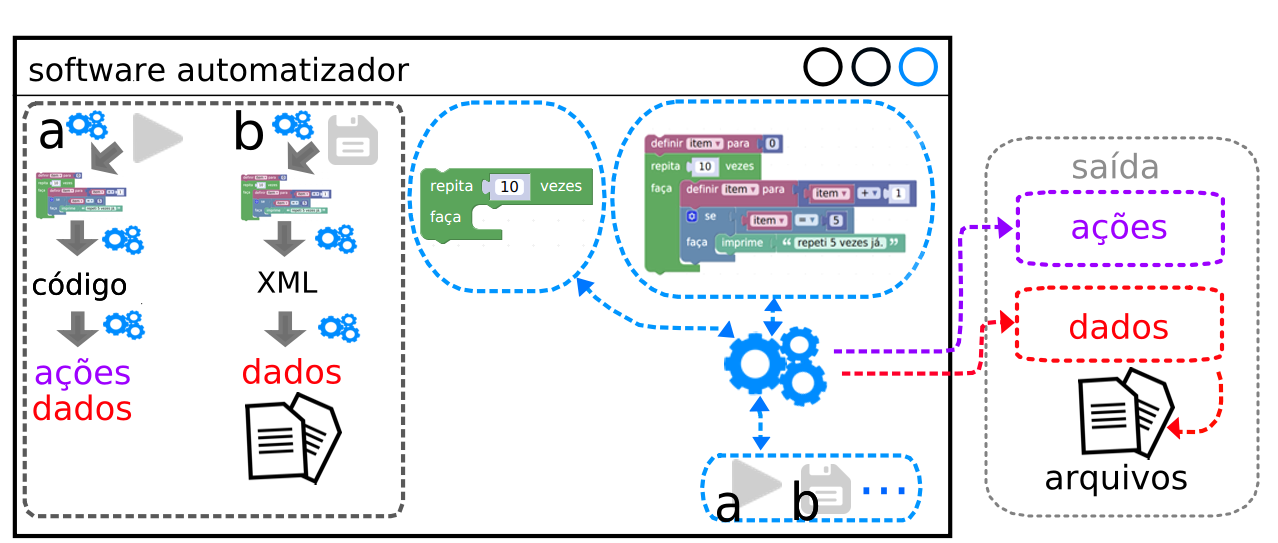
\includegraphics[width=1.0\textwidth]{imagens/blocklyDiagram}
                    \caption{Estrutura geral da solução.}
                    \label{fig:blocklyDiagram}}
                \end{figure}

                Alem dos diversos blocos já existentes na biblioteca, úteis para a definição de repetições, variáveis como textom números e listas, lógica e operações, para adaptar o blockly ao contexto de automação, serão desenvolvidos mais 4 bloco fundamentais para a automação, observando os requisitos elencados, dentro da abordagem de captura e execução já discutidods:

                \begin{itemize}
                    \item Um bloco que permite realizar clique simples em uma área da tela.
                    \item Outro que permite realizar clique duplo em uma área da tela
                    \item Um que permite esperar por um evento dentro do contexto de captura e execução, procurando a cada tanto intervalo de tempo definido pelo usuário
                    \item Por último, outro bloco que permita digitar valores que possam ser convertidos para texto, como números, texto em sí ou variáveis cujo valor possam ser convertidas para texto.
                \end{itemize}

            \subsection {Ações do software automatizador}

            \subsection {Codificação}

                Como escopo foram delimitados alguns pré-requisitos necessários para codificar o software modelado dentro das abordagens já tratadas, onde, o software deve ser uma aplicação desenvolvida usando Java e JavaScript. Devido ao fato de que a biblioteca blockly é desenvolvida em JavaScript e também, levando em consideração que a linguagem Java é uma linguagem robusta para lidar com a abordagem de cliente/servidor em aplicações web permitindo melhor integração com a biblioteca Blockly que por sua natureza executa em ambiente web como uma aplicação cliente, portanto, o automatizador trabalhará como um servidor que irá rodar, controlar e apresentar uma página web com a workspace da biblioteca Blockly injetada como uma aplicação web.

                \subsubsection {Integração do blockly em uma aplicação Java}

                    Em um primeiro momento, com o objetivo de rodar o Blockly, uma biblioteca JavaScript 100\% \emph{client side} dependente de um ambiente web, em uma aplicação java, optou-se por uma solução que envolve uma aplicação JavaFX com um cliente \emph{web} embutido, descrita de forma geral na imagem \ref{fig:struct}.

                    \begin{figure}[!htb]
                        {\centering
                        \includegraphics[width=1.0\textwidth]{imagens/struct.png}
                        \caption{Estrutura geral da solução.}
                        \label{fig:struct}}
                    \end{figure}

                    O software ao iniciar carrega a página da aplicação web desenvolvida com base na biblioteca Blockly em uma instância da classe \texttt{WebEngine}, contida na plataforma JavaFX, sendo que esta instância pertencente a um objeto da classe \texttt{WebView} também oriunda da plataforma JavaFX, responsável pela gestão e renderização da página \emph{web} na interface gráfica de uma aplicação JavaFX.

                    Foi utilizada a funcionalidade LiveConnect, presente na maioria dos navegadores web, que permite a comunicação entre o navegador e aplicativos java para conectar o software e a aplicação web. Foi desenvolvida a classe \texttt{JavascriptMsgr} com o objetivo de estabelecer os métodos de comunicação entre a aplicação web e o software, contendo uma referência para o objeto instanciado da classe \texttt{javafx.scene.web.WebEngine} com o qual cria um objeto \texttt{netscape.javascript.JSObject} que torna a classe \texttt{JavascriptMsgr} visível para a aplicação \emph{web}.

                    A classe \texttt{JavascriptMsgr} trata tanto as mensagens vindas da aplicação \emph{web} como as mensagens enviadas do software, a imagem \ref{code:javascriptmsg.java} apresenta dois exemplos de métodos presentes na classe \texttt{JavascriptMsgr} em trechos distintos\footnote{código completo disponível em https://github.com/RomuloPBenedetti/TCC/tree/master/Software/src/}, onde o primeiro envia uma mensagem para a aplicação web e o segundo recebe uma mensagem.


                    \begin{figure}[!htb]
                    \begin{lstlisting}
                        // método que envia uma String contendo o arquivo XML gerado na ultima vez em que foi
                        // salvo a blockly.mainWorkspace

                        public void loadBlocks(String xml) {
                            com.sun.javafx.application.PlatformImpl.runAndWait(() ->{
                                String escaped = StringEscapeUtils.escapeEcmaScript(xml);
                                engine.executeScript("loadBlocks(\""+ escaped +"\")");
                            });
                        }

                        // método que recebe um pedido para esperar enquanto não localizar uma imagem na
                        // pasta raiz, recebe um endereço relativo na pasta raiz do software e um valor
                        // de intervalo em milissegundos que deve esperar a cada procura sem sucesso
                        public void waitImg (String imgSrc, int milisec){
                            try {
                                BufferedImage target = null;
                                target = ImageIO.read(new File(imgSrc.substring(3)));
                                BufferedImage screenshot =
                                    robot.createScreenCapture(primaryScreenBounds);
                                ImageSearch is = new ImageSearch(target);

                                while(is.search(screenshot)[0] == -1){
                                    screenshot = robot.createScreenCapture(primaryScreenBounds);
                                    System.out.println("tried");
                                    Thread.sleep(milisec);
                                }
                                System.out.println("match!");
                            } catch (IOException | InterruptedException e) {
                                e.printStackTrace();
                            }
                        }
                    \end{lstlisting}
                        \caption{Dois métodos da classe mediadora da comunicação entre a aplicação web e o software}
                    	\label{code:javascriptmsg.java}
                    \end{figure}

                    A classe possui diversos métodos que estendem as funcionalidades da aplicação \emph{web} e permitem ao software utilizar a biblioteca blockly para fornecer a biblioteca visual, gerar e executar código.

                \subsubsection {Interação e pesquisa por regiões na tela do sistema operacional}

                    A interação com o Sistema operacional é realizada por instâncias da classe \texttt{java.awt.Robot} capaz de gerar eventos de sistema, nativos. Apesar de ter sido desenvolvida com o objetivo principal de realizar testes automatizados e aplicações autoexecutáveis, por ser capaz de manipular \emph{mouse} e teclado em nível de sistema, pode ser utilizada para qualquer tarefa que busque automatizar o controle do sistema operacional.

                    Para encontrar as áreas a serem clicadas ou regiões a serem observadas na espera de uma mudança, foi desenvolvida a classe \texttt{ImageSearch} com uma solução própria de pesquisa otimizada para imagens, que analisa uma imagem capturada da tela do sistema em busca de referências exatas das áreas escolhidas pelos usuários.

                    Diversas outras soluções foram analisadas como a biblioteca OpenCV~\cite{openCV} ou ainda o \emph{framework} brasileiro de processamento de imagens em Java, Marvin~\cite{marvin}. Porém outras soluções traziam diversos problemas que não se justificavam, variando da necessidade de mais bibliotecas, adaptação a uma abordagem mais complicada e distante da necessidade do projeto ou ainda limitações em termos de plataformas.

                    A abordagem é descrita na figura \ref{fig:ImageSearch}, se trata de extrair da área selecionada pelo usuário, dois \emph{pixels}, um com o maior valor de cor RGB dentre todos e outro com o menor valor dentre todos, assim como a distância 'x' e 'y' destes dois \emph{pixels} da origem. Por questões de otimização as cores nas imagens são analisadas como se fossem inteiros absolutos de 32 bits.

                    Posteriormente percorre quase todos os \emph{pixels} da imagem capturada da tela do sistma, de x = 0 até x = (larguraCaptura - larguraArea), usando a posição em que se encontra como âncora para verificar nas posições salvas dos \emph{pixels} extraídos da área são iguais aos \emph{pixels} na posição da imagem.

                    Caso os 2 \emph{pixels} sejam iguais, inicia-se uma análise de uma malha esparsa de \emph{pixels} na área, onde é somado a diferença dos \emph{pixels} da imagem extraída pelo usuário e a imagem capturada da tela, caso a diferença no final for zero, significa que foi encontrado uma área na imagem capturada igual à imagem da área que o usuário escolheu e neste caso a função retorna a posição 'x' 'y' da âncora.

                    Os métodos principais da classe \texttt{ImageSearch}\footnote{código completo disponível em https://github.com/RomuloPBenedetti/TCC/tree/master/Software/src/}, podem ser observados na imagem \ref{code:ImageSearch.java}.

                    \begin{figure}[!htb]
                        {\centering
                        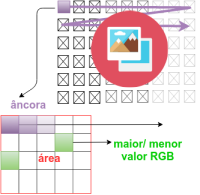
\includegraphics[width=0.3\textwidth]{imagens/searchImage.png}
                        \caption{descrição visual da tarefa realizada pela classe \texttt{ImageSearch}.}
                        \label{fig:ImageSearch}}
                    \end{figure}

                    \begin{figure}[!htb]
                    \begin{lstlisting}

                        public final void storeTarget(BufferedImage t) {
                        this.t = t; int rgb; tWidth = t.getWidth(); tHeight = t.getHeight();
                        for(int x = 0; x < tWidth; x++) {
                            for (int y = 0; y < tHeight; y++) {
                                rgb = t.getRGB(x, y);
                                if (Integer.compareUnsigned(rgb, max)>0) { max = rgb; maxX = x; maxY = y; }
                                if (Integer.compareUnsigned(rgb, max)<0) { min = rgb; minX = x; minY = y; }
                            }
                        }
                    }

                    public final int[] search(BufferedImage i) {

                        int iWidth, iHeight, point[] = new int[2];
                        point[0] = -1; point[1] = -1;
                        int startX[] = new int[cores], endX[] = new int[cores];
                        int startY[] = new int[cores], endY[] = new int[cores];

                        iWidth = i.getWidth()-tWidth; iHeight = i.getHeight()-tHeight;
                        ExecutorService executor = Executors.newFixedThreadPool(cores);

                        for (int q = 0 ; q < cores ; q++){
                            startX[q] = (iWidth/cores)*q; startY[q] = 0;
                            endX[q] = (iWidth/cores)*(q+1); endY[q] = iHeight;
                            int fQuad = q;

                            executor.execute(() -> {
                                Thread.currentThread().setName("thread" + fQuad);
                                int difference = 100; int rgbC;
                                for (int x = startX[fQuad]; x < endX[fQuad]; x++) {
                                    for (int y = startY[fQuad]; y < endY[fQuad]; y++) {
                                        rgbC = i.getRGB(x + maxX, y + maxY);
                                        if (rgbC == max) {
                                            rgbC = i.getRGB(x + minX, y + minY);
                                            if (rgbC == min) {
                                                difference = 0;
                                                for (int ty = 0; ty < tHeight; ty = ty +3) {
                                                    for (int tx = 0; tx < tWidth; tx = tx +3) {
                                                        difference += t.getRGB(tx, ty) - i.getRGB(x+tx, y+ty);
                                                    }
                                                }
                                                if (difference == 0) {
                                                    point[0] = x; point[1] = y;
                                                    executor.shutdownNow();
                                                }
                                            }
                                        }
                                        if (difference == 0) break;
                                    }
                                    if (difference == 0) break;
                                }
                            });
                        }
                        try {
                            executor.awaitTermination(1, TimeUnit.SECONDS);
                        } catch (InterruptedException e) {
                            e.printStackTrace();
                        }
                        return point;
                    }
                    \end{lstlisting}
                        \caption{Métodos que analisam a imagem da área e a imagem capturada da tela do sistema}
                    	\label{code:ImageSearch.java}
                    \end{figure}

                    O método \texttt{StoreTarget} percorre a imagem que o usuário selecionou para ser clicada ou analisada e compara o valor de cada \emph{pixel} com variáveis auxiliares, onde posteriormente sobrescreve o valor destas variáveis se o \emph{pixel} for realmente um valor maior ou menor do que os considerados anteriormente.

                    Já o método \texttt{search} procura pelo máximo ou mínimo na imagem capturada pelo software, quando encontra a área que contem nas mesmas posições o valor máximo e mínimo, analisa a área um pixel a cada três, caso a soma de todas as diferenças da área de um valor 0 todas as \emph{threads} são paradas e a posição do \emph{pixel} âncora ou origem da área é retornado. A tarefa também é dividia entre os núcleos do processador do usuário para obter melhor performance e o método apenas retorna quando o todas as \emph{threads} iniciadas pela pesquisa terminarem.

                \subsubsection {Utilização e adaptação do blockly para automação}

                    Para fornecer as funcionalidades foram definidos quatro blocos que expressam funcionalidades fundamentais para a automatização, dois blocos que expressam a habilidade de clicar em algum lugar da interface, um para clique duplo e outro para clique único, também, um bloco que permite esperar por algum evento visual, para que seja possível esperar a finalização do processamento dos modelos, e por último um bloco que permite digitar texto na entrada de texto do sistema operacional.

                    É possível observar os blocos na imagem \ref{fig:myblocks} e a descrição formal em JavaScript destes blocos na figura \ref{code:myBlocks.js}\ref{code:myBlocksGenerator.js}\footnote{código completo disponível em https://github.com/RomuloPBenedetti/TCC/tree/master/Software/src/}.


                    \begin{figure}[!htb]
                    \begin{lstlisting}
                        Blockly.Blocks['click_single_special'] = {
                          init: function() {
                            this.appendDummyInput("imageInput")
                                .appendField("clicar uma vez em:")
                                .appendField(new Blockly.FieldImageButton("../images/icons/clickBlack.png", 30, 30, "", imageButtonEvent), "FieldImageButton");
                            this.setPreviousStatement(true, null);
                            this.setNextStatement(true, null);
                            this.setColour(60);
                            this.setTooltip('Procura na sua tela pela região que a imagem representa e clica no centro uma veze, para escolher, clique na imagem branca do bloco, va ao local desejado aperte ctrl+shift+c, selecione onnde clicar com o mouse e aperte enter.');
                          }
                        };

                        Blockly.Blocks['click_doble_special'] = {
                          init: function() {
                            this.appendDummyInput("imageInput")
                                .appendField("clicar duas vezes em:")
                                .appendField(new Blockly.FieldImageButton("../images/icons/clickBlack.png", 30, 30, "", imageButtonEvent), "FieldImageButton");
                            this.setPreviousStatement(true, null);
                            this.setNextStatement(true, null);
                            this.setColour(60);
                            this.setTooltip('Procura na sua tela pela região que a imagem representa e clica no centro duas vezes, para escolher, clique na imagem branca do bloco, va ao local desejado aperte ctrl+shift+c, selecione onnde clicar com o mouse e aperte enter.');
                            console.log(this.id);
                          }
                        };

                        Blockly.Blocks['text_typer'] = {
                          init: function() {
                            this.appendDummyInput("textToType")
                                .appendField("digitar:")
                                .appendField(new Blockly.FieldTextInput("texto"), "text");
                            this.setPreviousStatement(true, null);
                            this.setNextStatement(true, null);
                            this.setColour(60);
                            this.setTooltip('');
                            this.setHelpUrl('http://www.example.com/');
                          }
                        };

                        Blockly.Blocks['Image_Wait'] = {
                          init: function() {
                            this.appendDummyInput("imageInput")
                                .appendField("esperar enquanto não encontrar:")
                                .appendField(new Blockly.FieldImageButton("../images/icons/clickBlack.png", 30, 30, "", imageButtonEvent), "FieldImageButton");
                            this.appendValueInput("miliToWait")
                                .setCheck("Number")
                                .setAlign(Blockly.ALIGN_RIGHT)
                                .appendField("procurando a cada:");
                            this.appendDummyInput()
                                .appendField("milisegundos");
                            this.setInputsInline(true);
                            this.setPreviousStatement(true, null);
                            this.setNextStatement(true, null);
                            this.setColour(60);
                            this.setTooltip('para escolher por que imagem esperar, clique na imagem branca do bloco, va ao local desejado aperte ctrl+shift+c, selecione onnde clicar com o mouse e aperte enter.');
                            this.setHelpUrl('http://www.example.com/');
                          }
                        };
                    \end{lstlisting}
                        \caption{Descrição dos blocos na aplicação web e seus respectivos geradores de código}
                        \label{code:myBlocks.js}
                    \end{figure}

                    \begin{figure}[!htb]
                    \begin{lstlisting}
                        Blockly.JavaScript['click_doble_special'] = function(block) {
                          src = (block.getFieldValue('FieldImageButton')).replaceAll("\\\\","\\\\");
                          running = 'if (running) {\n';
                          calling = '    running = java.clickIn(\"' + src + '\",' + 2 + ');\n';
                          end =     '}\n';
                          var code = running + calling + end;
                          return code;
                        };

                        Blockly.JavaScript['click_single_special'] = function(block) {
                          src = (block.getFieldValue('FieldImageButton')).replaceAll("\\\\","\\\\");
                          running = 'if (running) {\n';
                          calling = "java.clickIn(\"" + src + '\",' + 1 + ');\n';
                          end =     '}\n';
                          var code = running + calling + end;
                          return code;
                        };

                        Blockly.JavaScript['text_typer'] = function(block) {
                          text = block.getFieldValue('text');
                          running = 'if (running) {\n';
                          calling = "    running = java.type(\"" + text + '\");\n';
                          end =     '}\n';
                          var code = running + calling + end;
                          return code;
                        };

                        Blockly.JavaScript['Image_Wait'] = function(block) {
                          src = (block.getFieldValue('FieldImageButton')).replaceAll("\\\\","\\\\");
                          milisec = Blockly.JavaScript.valueToCode(block, 'miliToWait', Blockly.JavaScript.ORDER_ATOMIC) || '0'
                          running = 'if (running) {\n';
                          calling = '    java.waitImg(\"' + src + '\", '+ milisec + ');\n';
                          end =     '}\n';
                          var code = running + calling + end;
                          return code;
                        };
                    \end{lstlisting}
                        \caption{Geradores de código java dos blocos construidos}
                        \label{code:myBlocksGenerator.js}
                    \end{figure}

                    Como é possível ver o bloco \texttt{Image\_Wait} e os blocos que representam as ações de clique de mouse, \texttt{click\_doble\_special} e \texttt{click\_single\_special} utilizam um campo próprio chamado \texttt{FieldImageButton}, desenvolvido observando-se o campo original presente na biblioteca Blockly \texttt{field\_image}\footnote{o código desta classe pode ser encontrado em https://github.com/google/blockly/}, este campo adiciona a imagem um \emph{eventListenner} que ao ser clicado envia uma mensagem que dá início a tarefa de captura de tela no software, que ao ser terminada pelo usuário, envia uma mensagem contendo o caminho da imagem da área selecionada pelo usuário que deve sofrer a ação do bloco junto com suas dimensões. Por sua vez a aplicação web atualiza a imagem do bloco para representar a área que o usuário escolheu.

                    Toda a tarefa é mantida coêsa transferindo junto com estas mensagens o ID único que a própria biblioteca Blockly gera para cada bloco assim tanto a aplicação web como o software sempre sabem para que bloco é cada mensagem. Por questões de flexibilidade e simplicidade foi decidido utilizar a linguagem JavaScript por questões de simplicidade já que é uma das linguagens nativas do software e disponível para os outros blocos da biblioteca por padrão já.

                    Quando o usuário clica no botão para executar o modelo no software, é enviado uma mensagem para a aplicação web, pedindo que para que a biblioteca Blockly monte o código com base no quebra-cabeça montado e por fim, execute o código com a função \texttt{eval}.

                    Como é possível observar, os geradores de código foram construídos para realizar chamadas no no software java e portanto, a aplicação web fica responsável apenas pela montagem da lógica que guia a execução das tarefas tais como construção de repetições ou definições de valores a serem enviados junto as mensagens para que o software as realize. É possível ver um exemplo do código gerado por um conjunto de blocos nas figuras \ref{fig:blocosecodigo}.\ref{code:blocosecodigo.js}.

                    \begin{figure}[!htb]
                        {\centering
                        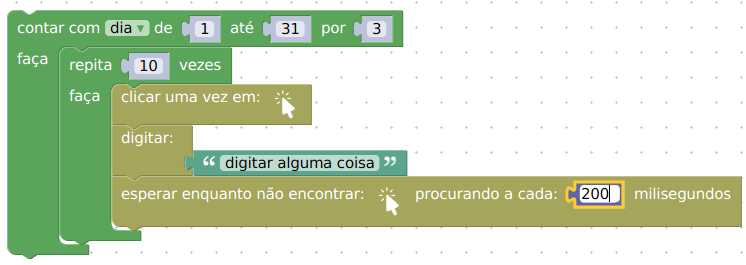
\includegraphics[width=1.0\textwidth]{imagens/blocosecodigo.png}
                        \caption{Exemplo de um quebra-cabeça}
                        \label{fig:blocosecodigo}}
                    \end{figure}

                    \begin{figure}[!htb]
                    \begin{lstlisting}
                        var running = true; var dias;

                        for (dias = 1; dias <= 31; dias += 3) {
                          for (var count = 0; count < 10; count++) {
                            if (running) {
                            java.clickIn("../images/icons/clickBlack.png",1);
                            }
                            if (running) {
                                running = java.type("digitar alguma coisa");
                            }
                            if (running) {
                                java.waitImg("../images/icons/clickBlack.png", 200);
                            }
                          }
                        }
                    \end{lstlisting}
                        \caption{Exemplo do código gerado por este quebra-cabeça}
                        \label{code:blocosecodigo.js}
                    \end{figure}

        \chapter {Resultados}

            \section {O software automatizador}

                O produto final deste projeto, o software automatizador, possui uma interface sucinta, contida dentro da definição dos componentes que foram modelados para interação do usuário durante seu planejamento. O principal objetivo da quantia reduzida de elementos consiste em reduzir as interações dentro do possível considerando os requisitos e objetivos do projeto, para assim, reduzir o tempo gasto compreendendo apenas a interface do software e logo o usuário começar a estudar e compreender o quanto antes possível, como funcionam os blocos e como montar uma automação, tarefa que ainda demanda capacidade lógica. É possível ver a interface na figura \ref{fig:app}.

                existem, quatro botões principais na interface: a lixeira, para onde o usuário pode arrastar o quebra-cabeças para descartá-lo, um para executar a simulação que se encontra montada atualmente, um para carregar um quebra-cabeças que tenha sido salvo e outro para salvar em um arquivo XML um quebra-cabeças atualmente montado no automatizador.

                Além destes quatro botões, existem os tres botões na parte superior da janela responsáveis por fechar, maximizar ou minimizar a janela. Na mesma altura, nas proximidades destes três botões, a ceta do mouse muda de simbolo, indicando que nesta região, é possível clicar e segurar para mover a janela.

                Próximo aos quatro botões principais na interface ainda temos mais tres botões, um circulo com um ponto dentro, que quando clicado centraliza a área de edição no quebra-cabeças atual, e dois circulos, um com o simbolo de soma e outro com o simbolo de subtração, com os quai é possível aumentar ou reduzir a visão do quebra-cabeças na área de edição, para que a visualização fique mais confortável dependendo do tamanho do quebra-cabeças.

                \begin{figure}[!htb]
                    {\centering
                    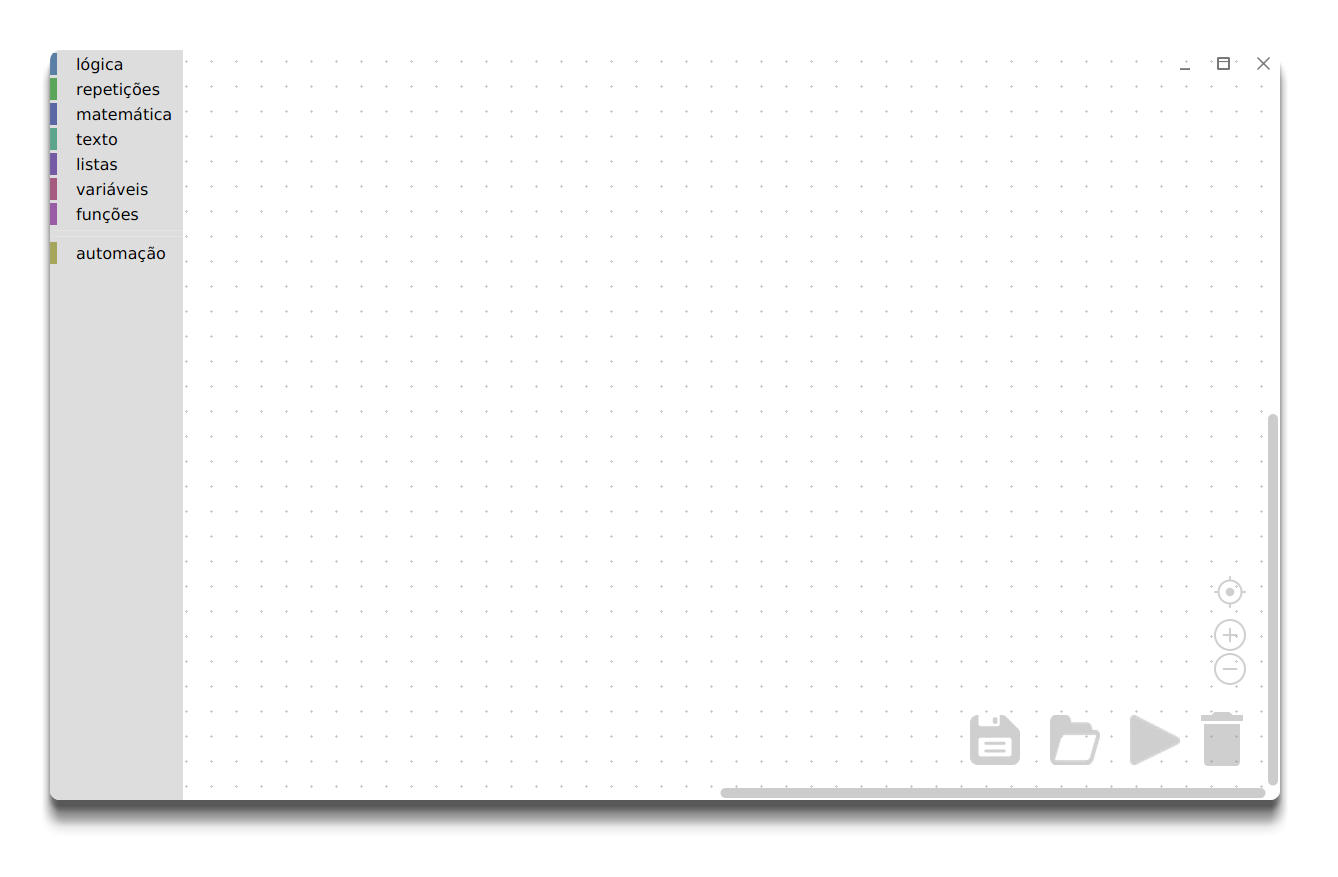
\includegraphics[width=1.0\textwidth]{imagens/app.png}
                    \caption{Tela inicial do software desenvolvido}
                    \label{fig:app}}
                \end{figure}

                Além dos botões descritos, temos a área de trabalho, onde a automação é montada, um espaço em branco com uma grade pontilhada, e também temos os elementos de automação armazenados em oito categorias no painel cinza a esquerda, que são:

                \begin{itemize}
                    \item lógica:
                    \item repetições:
                    \item matemática:
                    \item texto:
                    \item listas:
                    \item variáveis:
                    \item funções:
                    \item automações:
                \end{itemize}

                Para utilizar um dos blocos basta clicar e segura-lo, arrastando para a área de trabalho e soltando em uma área em branco ou alinhado com o encaixe adequado de algum bloco já existente na área de trabalho, para que se encaixem.

                Das oito categorias apresentadas, a categoria "automações" contem os blocos desenvolvidos neste projeto, que permitem automatizar outros softwares. Os blocos podem ser observados na figura \ref{fig:myblocks}, que, após carregados na área de trabalhopodem ser configurados.

                Para selecionar aa imagem que representa a área onde será clicado ou pela qual será esperado, o usuário deve clicar no simbolo da ceta de mouse no bloco. o monitor do computador será envolvido por uma linha pontilhada vermelha, indicando que o mesmo pode minimizar, mover ou interagir com o sistema em busca da imagem do local onde clicar ou pelo qual esperar. Assim que encontrado, o usuário pode ativar o comando de teclado ctrl+shift+c para capturar uma imagem da tela atual, posteriormente clicando e arrastando para selecionar uma área retangular onde os blocos de clique irão clicar no centro e, no caso do bloco de espera irá procurar.

                O bloco de espera irá procurar pela imagem na tela a cada tantos milissegundos que o usuário pode definir inserindo um bloco do tipo número contido na categoria matemática.

                Já o bloco digitar, permite a conexão de qualquer tipo de bloco que devolva um valor, tal como números e textos, que será posterior digitado quando a automação chegar neste bloco.

                \begin{figure}[!htb]
                    {\centering
                    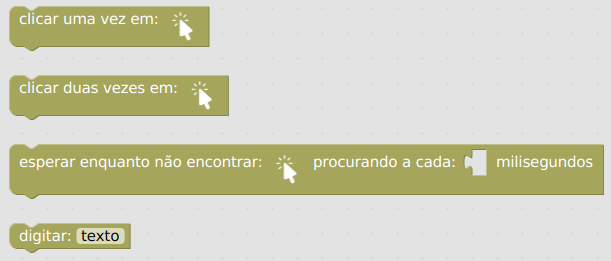
\includegraphics[width=1.0\textwidth]{imagens/blocks.png}
                    \caption{Blocos construídos para as operações de automação}
                    \label{fig:myblocks}}
                \end{figure}


                Outras formas de interação possíveis no software são, clicando e arrastando a área de trabalho para move-la ou ainda usando o botão deletar do teclado para deletar um conjunto ou um bloco selecionado. Também é possível utilizar o comando ctrl+z para desfazer alterações como deleção de blocos.

            \section {Exemplos simples de automações}

                Para melhor compreender o funcionamento do software serão apresentados dois quebra cabeças simples.

            \section {Validando a solução com os casos de teste}

            Com as funcionalidades desenvolvidas no software não é possível solucionar todas as questões desenvolvidas nos casos de teste dos 3 modelos Porem é possível solucionar em geral o problema dos modelos projetando o quebra-cabeças levando em consideração as limitações do software.

            % adicionado após entrega do projeto final
            Algumas limitações principais encontradas ao modelar um quebra-cabeças para os casos de teste coletados foram:

            \begin{itemize}
                \item O software não é capaz de suavizar a criticidade com a qual procura os campos a serem clicados, logo qualquer diferença já torna impossível para o software localizar o campo novamente.
                \item O software não é capaz de se deslocar pela interface do sistema operacional, ir para a área de trabalho ou navegar entre as janelas abertas do sistema.
                \item O software não é capaz de editar arquivos de texto. Embora possua diversas capacidades para processar textos dentre seus blocos, não ha nenhum bloco capaz de abrir um arquivo armazenado em alguma pasta do sistema ou ainda ler texto da tela.
                \item Apesar de ser capaz de esperar por mudanças gráficas na tela, o software não é capaz de tomar decisões lógicas na ocorrência de uma mudança gráfica, habilidade relevante para o tratamento de erros ou seguimento de múltiplos fluxos.
            \end{itemize}

            Dentre outras limitações não fundamentais, esta o fato de que o software não é capaz de pausar ou reiniciar simulações em andamento, assim como também não ha \emph{feedback} visual do software quando o mesmo finaliza a tarefa ou encontra algum erro.

            \subsection {Simanihot}

            Foi validada apenas a abstração lógica da linguagem visual modelando um quebra-cabeças para o caso de uso do modelo Simanihot onde todos os problemas fundamentais para a solução do problema proposto no caso de uso são solucionados dentro da lógica disponibilizada pelo conjunto de peças do software, como é possível ver na figura \ref{fig:simanibloco}.

            % adicionado após entrega do projeto final
            Em especial, é necessário configurar o quebra-cabeças para fechar e reabrir a aplicação, já que o software não possibilita definir um nível de similaridade das áreas a serem clicadas, esperando uma similaridade exata, o que não ocorre de simulação em simulação, já que a cada simulação o texto que se encontra nos campos de texto é diferente do anterior.

            \begin{figure}[!htb]
                {\centering
                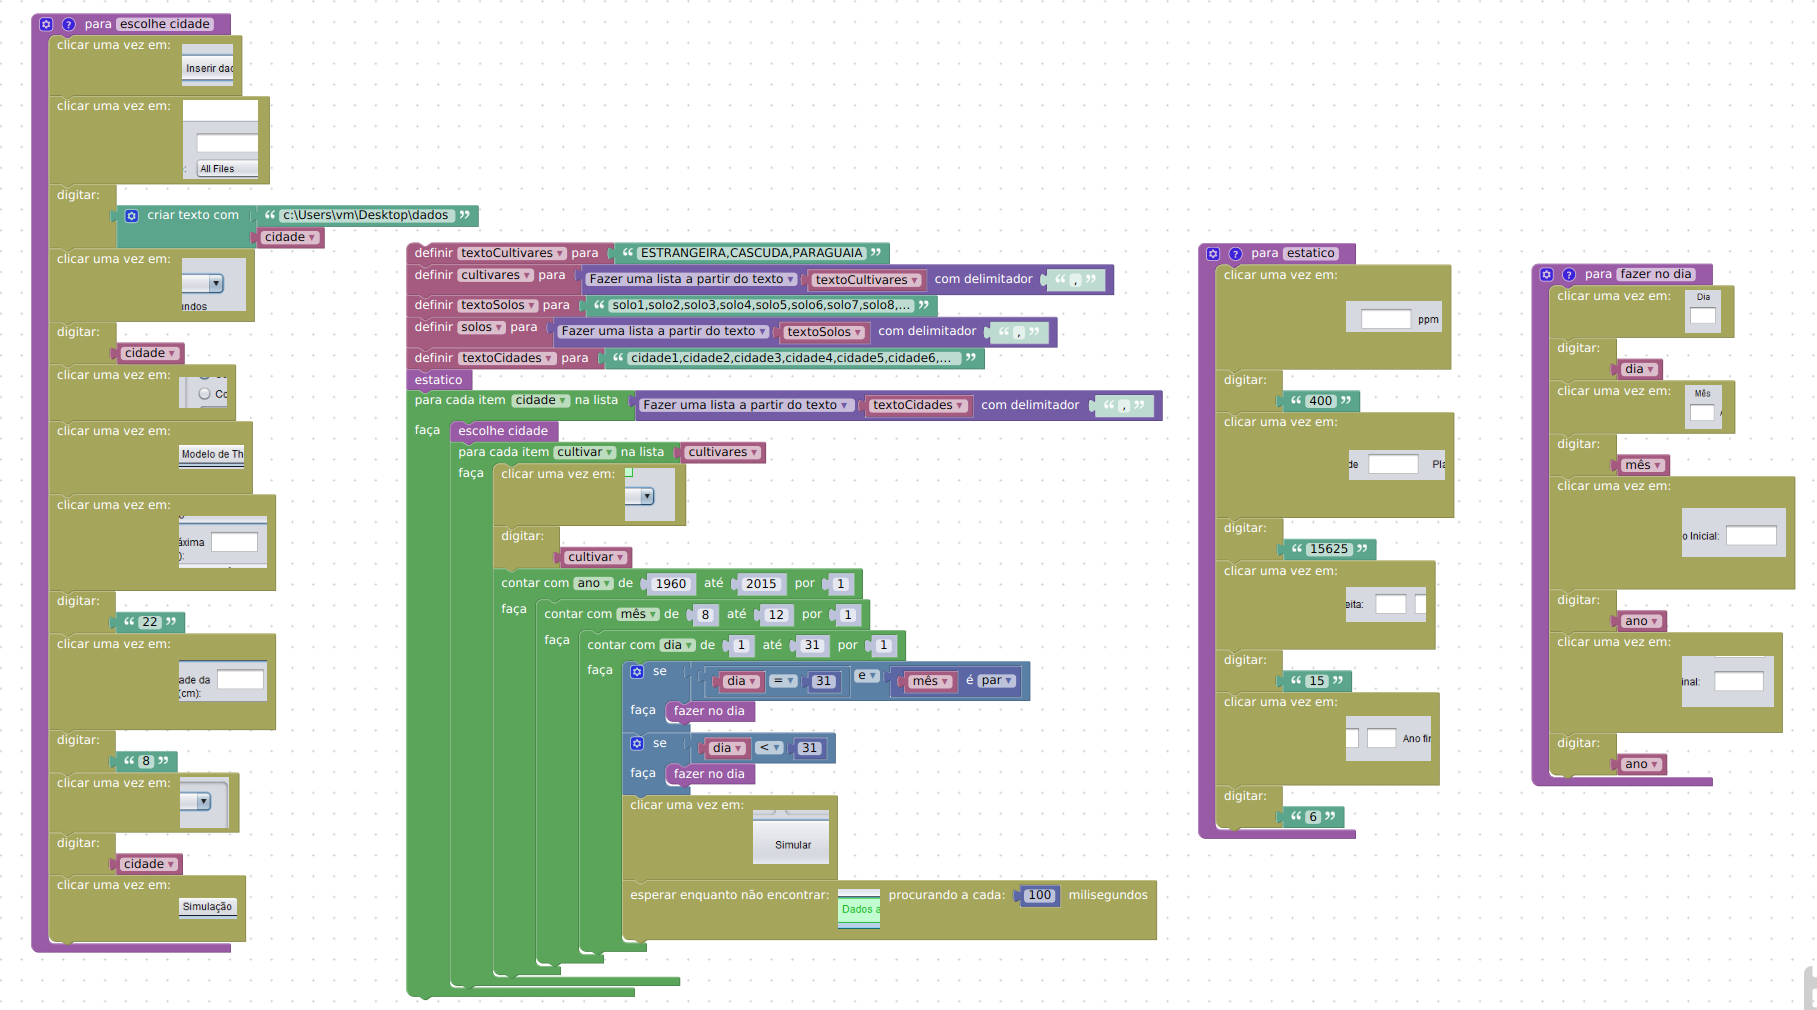
\includegraphics[width=1.0\textwidth]{imagens/simanihotBlock.png}
                \caption{Exemplo de um quebra-cabeça}
                \label{fig:simanibloco}}
            \end{figure}



        \chapter {Conclusão}

            A proposta inicial deste trabalho consistia principalmente em apresentar uma solução de automação de interfaces gráficas de forma simplificada com base na biblioteca de programação visual Blockly dentro do contexto de modelos de simulação de culturas agrícolas. Entretanto o resultado final desta pesquisa trata-se não de uma solução total dos problemas apresentados, mas de um software que oferece a possibilidade de automatização de alguns problemas com um escopo não tão grande como o dos problemas propostos, com base nas conclusões tomada durante o desenvolvimento, a partir dos percalços e da análise constante da amplitude da proposta e das necessidades durante a validação das abordagens em questão.

            Como contribuição este trabalho apresentou uma abordagem diferenciada na programação de tarefas automatizadas expondo de forma mais simplificada lógica comum em linguagens de programação e \emph{script} tradicionais, fornecendo uma ferramenta que pode descrever de forma muito flexível interações com a interface gráfica e permitindo em algum nível realizar a automatização de parte das tarefas maçantes presentes na interação com interfaces gráficas de modelos matemáticos de simulação de culturas agrícolas mais simples.

            A lista a seguir, não exaustiva, expõe em ordem de relevância, uma lista  de algumas melhorias que poderiam ser incorporadas em uma nova versão deste projeto:

            \begin{itemize}
            	\item Tratar arquivos com conteúdo de texto, permitindo copiar arquivos para outros locais, criar arquivos com novas informações, renomeá-los e processar e extrair informações destes textos.
                \item Refinar a forma com a qual o programa localiza e clica nos elementos gráficos, seja pela adição de procura por similaridades e áreas não exatas, ou por novos métodos para definição da área onde se deve clicar.
                \item Expandir a interação com o sistema operacional de forma que o software possa procurar dentre diversas janelas e na área de trabalho.
            	\item Fornecer \emph{feedback} visual ao finalizar automatizações ou receber erros durante a execução de uma automatização.
            	\item Obter uma forma mais eficiente de captura de tela já que a captura de tela realizada pela classe \texttt{Robot} além de lenta pode produzir artefatos e não capturar alguns elementos dinâmicos de alguns programas.
                \item Oferecer blocos que simplifiquem elementos lógicos já presentes na biblioteca Blockly permitindo a formulação de quebra-cabeças de automatização mais simples.
                \item Refinar os detalhes em geral da aplicação como salvamento e carregamento de quebra-cabeças de forma que sejam salvas também as imagens pré selecionadas, fornecimento de configurações para troca de idioma e possibilidade de pausar, continuar e reiniciar quebra-cabeças.
            \end{itemize}

	\setlength{\baselineskip}{\baselineskip}
	\bibliographystyle{abnt}
	\bibliography{andamento}
\end{document}
